\documentclass[a4paper, 14pt]{extarticle}
\usepackage[english,russian]{babel}
\usepackage[T1]{fontenc}
\usepackage[utf8]{inputenc}
\usepackage{fontspec}
\usepackage{indentfirst}
\usepackage{enumitem}
\usepackage{graphicx}
\usepackage[
  left=20mm,
  right=10mm,
  top=20mm,
  bottom=20mm
]{geometry}
\usepackage{parskip}
\usepackage{titlesec}
\usepackage{xurl}
\usepackage{hyperref}
\usepackage{float}
\usepackage[
  figurename=Рисунок,
  labelsep=endash,
  justification=centering
]{caption}
\usepackage[outputdir=build, newfloat]{minted}
\usepackage{chngcntr}

\selectlanguage{russian}

\hypersetup{
  colorlinks=true,
  linkcolor=black,
  filecolor=blue,
  urlcolor=blue,
}

\renewcommand*{\labelitemi}{---}
\setmainfont{Times New Roman}
\setmonofont{JetBrains Mono}[
  SizeFeatures={Size=11},
]

\newenvironment{code}{\captionsetup{type=figure}}{}
\BeforeBeginEnvironment{code}{\bigskip}
\AfterEndEnvironment{code}{\bigskip}

\setminted{
  fontsize=\footnotesize,
}

\setlength{\parskip}{6pt}

\setlength{\parindent}{1.25cm}
\setlist[itemize]{itemsep=0em,topsep=0em,parsep=0em,partopsep=0em,leftmargin=2.0cm,wide}
\setlist[enumerate]{itemsep=0em,topsep=0em,parsep=0em,partopsep=0em,leftmargin=2.0cm,wide}

\renewcommand{\thesection}{\indent\arabic{section}.}
\renewcommand{\thesubsection}{\indent\thesection\arabic{subsection}.}
\renewcommand{\thesubsubsection}{\indent\thesubsection\arabic{subsubsection}.}

\titleformat{\section}{\normalfont\bfseries}{\thesection}{0.5em}{}
\titleformat{\subsection}{\normalfont\bfseries}{\thesubsection}{0.5em}{}
\titleformat{\subsubsection}{\normalfont\bfseries}{\thesubsubsection}{0.5em}{}

\titleformat*{\section}{\normalfont\bfseries}
\titleformat*{\subsection}{\normalfont\bfseries}
\titleformat*{\subsubsection}{\normalfont\bfseries}

\titlespacing{\section}{\parindent}{\parskip}{\parskip}
\titlespacing{\subsection}{\parindent}{\parskip}{\parskip}
\titlespacing{\subsubsection}{\parindent}{\parskip}{\parskip}

\begin{document}

\begin{titlepage}
  \vspace{0pt plus2fill}
  \noindent

  \vspace{0pt plus6fill}
  \begin{center}
    {
    \bfseries
    Министерство науки и высшего образования Российской Федерации
    {
    \scriptsize
    ФЕДЕРАЛЬНОЕ ГОСУДАРСТВЕННОЕ АВТОНОМНОЕ ОБРАЗОВАТЕЛЬНОЕ УЧРЕЖДЕНИЕ ВЫСШЕГО
    ОБРАЗОВАНИЯ
    }
    «Национальный исследовательский университет ИТМО»

    (Университет ИТМО)

    \begin{minipage}[t]{0.42\textwidth}
      \vspace*{0pt}
      \begin{flushright}
        Факультет

        Образовательная программа
      \end{flushright}
    \end{minipage}
    \begin{minipage}[t]{0.57\textwidth}
      \vspace*{0pt}
      \begin{flushright}
        Инфокоммуникационных технологий

        11.03.02 Программирование в инфокоммуникационных системах
      \end{flushright}
    \end{minipage}
    }

    \vspace{0pt plus5fill}

    \LARGE{
      ОТЧЕТ

      по лабораторной работе 4

      по дисциплине \textbf{<<Разработка баз данных>>}
    }
  \end{center}

  \vspace{0pt plus4fill}
  \begin{flushright}
    Выполнил: \textbf{студент группы K33211 Швалов Д. А.}

    Проверил: \textbf{ст. преподаватель Осетрова И.С.}
  \end{flushright}

  \vspace{0pt plus8fill}
  \begin{center}
    Санкт-Петербург

    2024
  \end{center}
\end{titlepage}

\setcounter{page}{2}

\linespread{1.5}
\renewcommand{\baselinestretch}{1.5}

\section*{\large{Лабораторная работа №4 <<Обработка данных>>}}

\section{Цель работы}

Обработка данных.

\section{Задачи, решаемые при выполнении работы}

\begin{enumerate}[leftmargin=*]
  \item Добавление данных.
  \item Обновление данных.
  \item Удаление данных.
  \item Создание недостающих связей.
\end{enumerate}

\section{Объект исследования}

Обработка данных в СУБД \foreignlanguage{english}{Microsoft SQL Server} с
помощью \foreignlanguage{english}{Microsoft SQL Server Management Studio
  (SSMS)}.

\section{Исходные данные}

\begin{itemize}
  \item методические указания к лабораторной работе;
  \item СУБД Microsoft SQL Server;
  \item Microsoft SQL Server Management Studio;
  \item база данных ApressFinancial.
\end{itemize}

\section{Выполнение работы}

\subsection{Первая задача}

\subsubsection{Создание сценария в Query Editor}

С помощью контекстного меню, как это показано на рисунке \ref{fig:task-1-1}, был
открыт редактор запросов с предопределенным кодом. В соответствии с заданием,
данный код был отредактирован таким образом, как показано на рисунке
\ref{fig:task-1-2}. Также была использована инструкция
<<\foreignlanguage{english}{SET QUOTED\_IDENTIFIER OFF}>> для того, чтобы строки
в двойных кавычках рассматривались как строковые литералы. После выполнения
данного кода появилось сообщение в таблицу <<\foreignlanguage{english}{Shares}>>
была добавлена новая строка.

\begin{figure}[H]
  \centering
  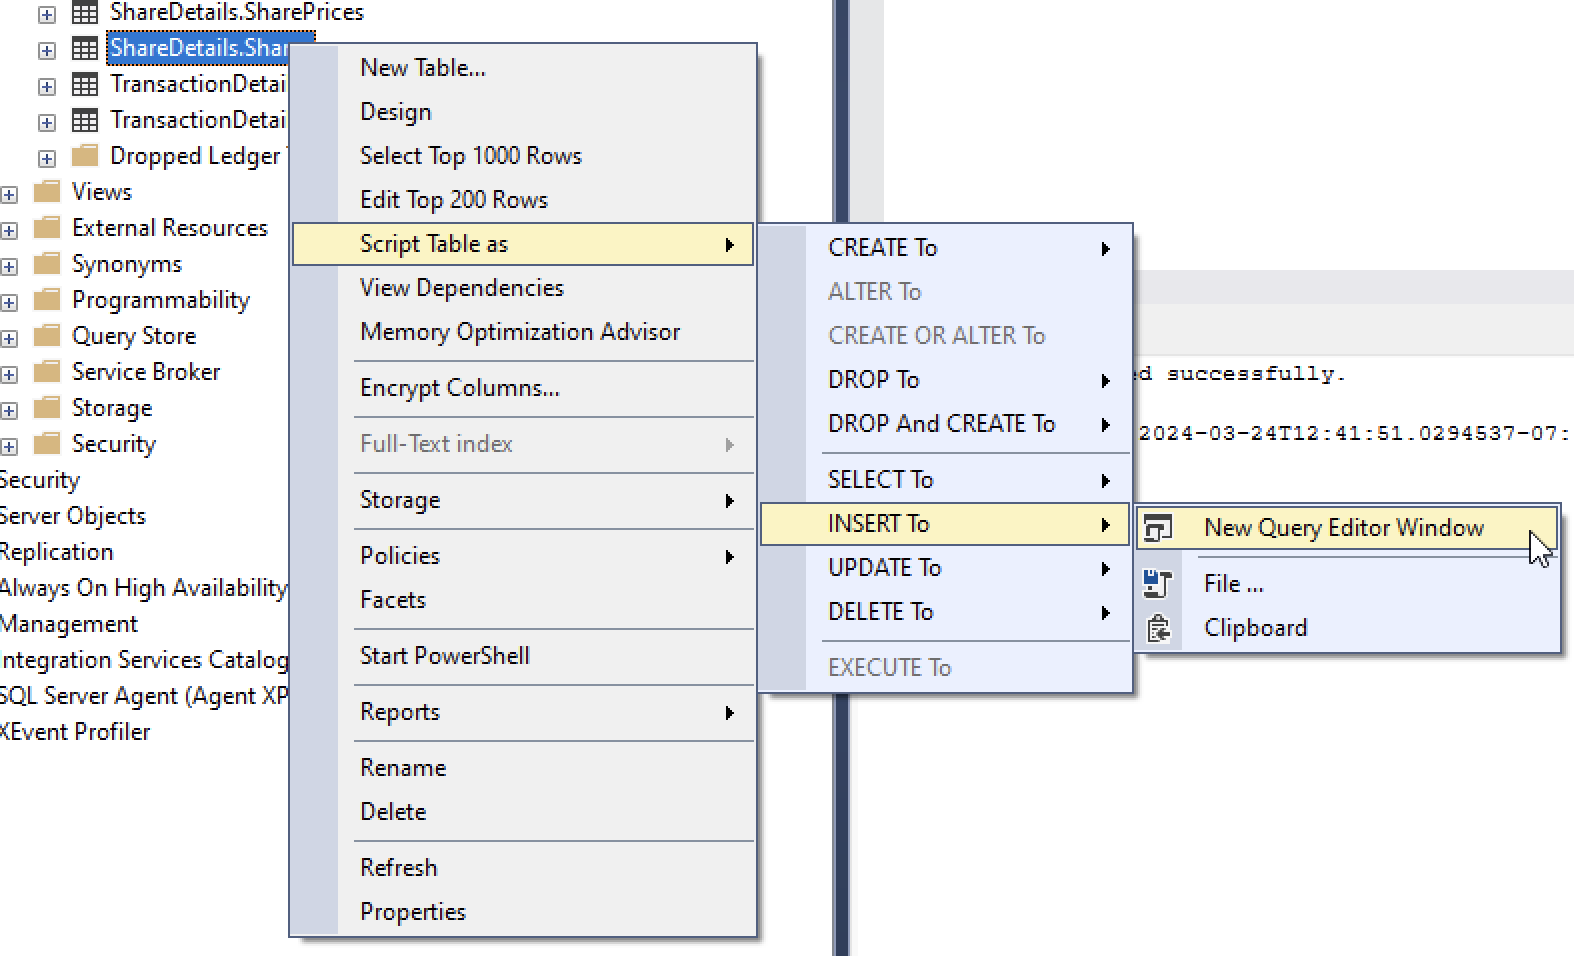
\includegraphics[width=0.8\textwidth]{images/task-1/1.png}
  \caption{Меню открытия редактора запросов}
  \label{fig:task-1-1}
\end{figure}

\begin{figure}[H]
  \centering
  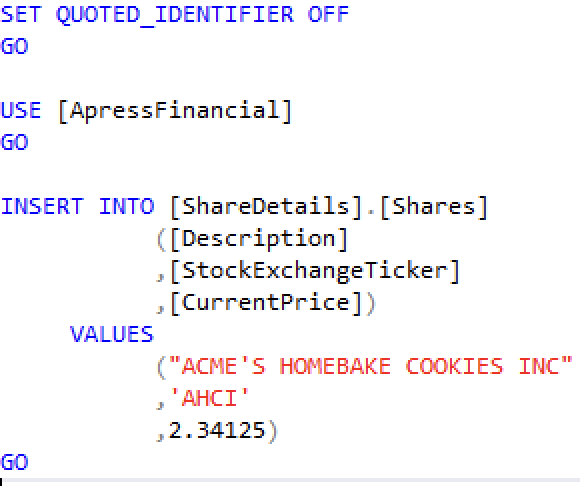
\includegraphics[width=0.6\textwidth]{images/task-1/2.png}
  \caption{Запрос добавления данных в таблицу
  <<\foreignlanguage{english}{Shares}>>}
  \label{fig:task-1-2}
\end{figure}

\subsubsection{Отметки NULL}

В свойствах столбцов таблицы <<\foreignlanguage{english}{Customers}>> было
проверено, что для поля <<\foreignlanguage{english}{CustomerId}>> свойство
<<\foreignlanguage{english}{Is Identity}>> установлено в
<<\foreignlanguage{english}{Yes}>> (рисунок \ref{fig:task-1-3}), а также, что
для поля <<\foreignlanguage{english}{DateOpened}>> указано значение по умолчанию
<<\foreignlanguage{english}{getdate()}>> (рисунок \ref{fig:task-1-4}). После
этого с помощью контекстного меню (рисунок \ref{fig:task-1-5}) было открыто окно
редактирования строк таблицы (\ref{fig:task-1-6}).

При попытке добавления строки с отсутствующими обязательными значениями для
столбцов, возникает ошибка, как показано на рисунке \ref{fig:task-1-7}. Все
столбцы, которые были помечены при создании таблицы как недопускающие пустых
значений, требуют обязательного заполнения. После корректного заполнения
столбцов, как это показано на рисунке \ref{fig:task-1-8}, новая строка была
успешно сохранена в базу данных. Также ей был присвоен идентификатор
<<\foreignlanguage{english}{CustomerId}>>, равный 6.

После этого в редакторе запросов был выполнен код, показанный на рисунке
\ref{fig:task-1-9}. В отличии от кода, выполненного в предыдущем задании, данный
код не содержит квадратных скобок в идентификаторах схем, таблиц и столбцов.

\begin{figure}[H]
  \centering
  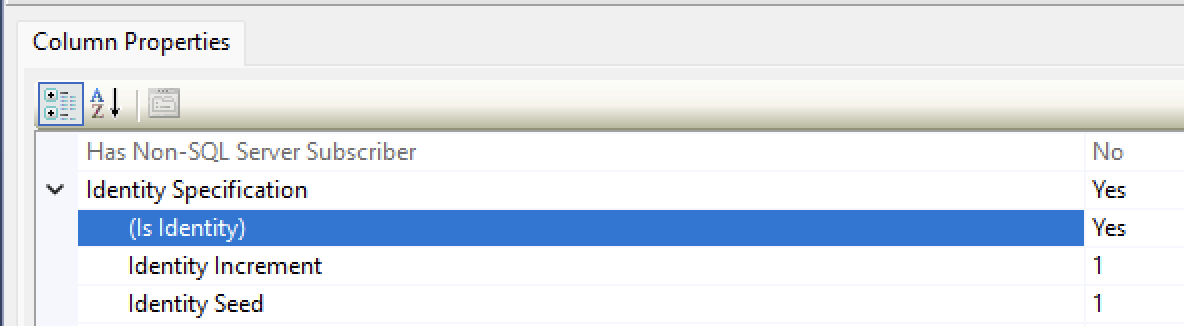
\includegraphics[width=\textwidth]{images/task-1/3.png}
  \caption{Свойства столбца <<\foreignlanguage{english}{CustomerId}>>}
  \label{fig:task-1-3}
\end{figure}

\begin{figure}[H]
  \centering
  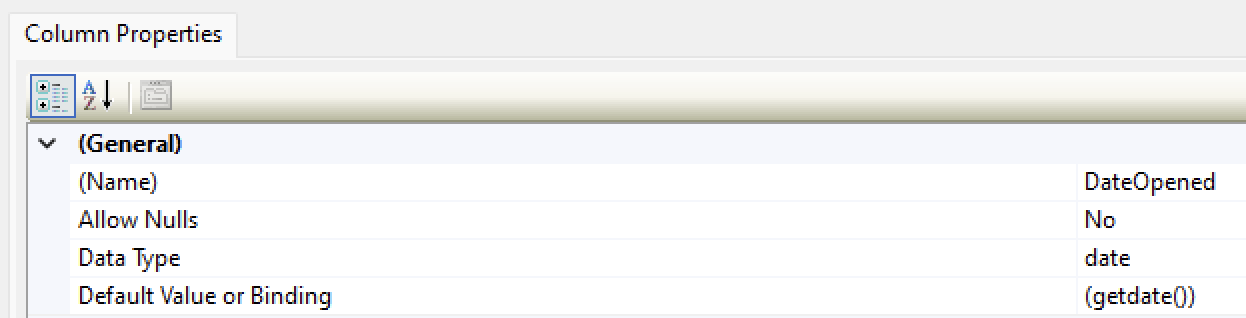
\includegraphics[width=\textwidth]{images/task-1/4.png}
  \caption{Свойства столбца \foreignlanguage{english}{DateOpened}}
  \label{fig:task-1-4}
\end{figure}

\begin{figure}[H]
  \centering
  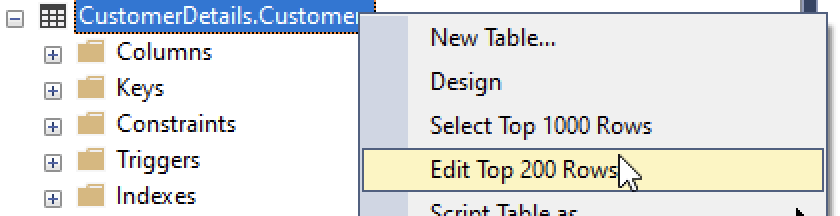
\includegraphics[width=0.7\textwidth]{images/task-1/5.png}
  \caption{Меню открытия окна редактирования строк}
  \label{fig:task-1-5}
\end{figure}

\begin{figure}[H]
  \centering
  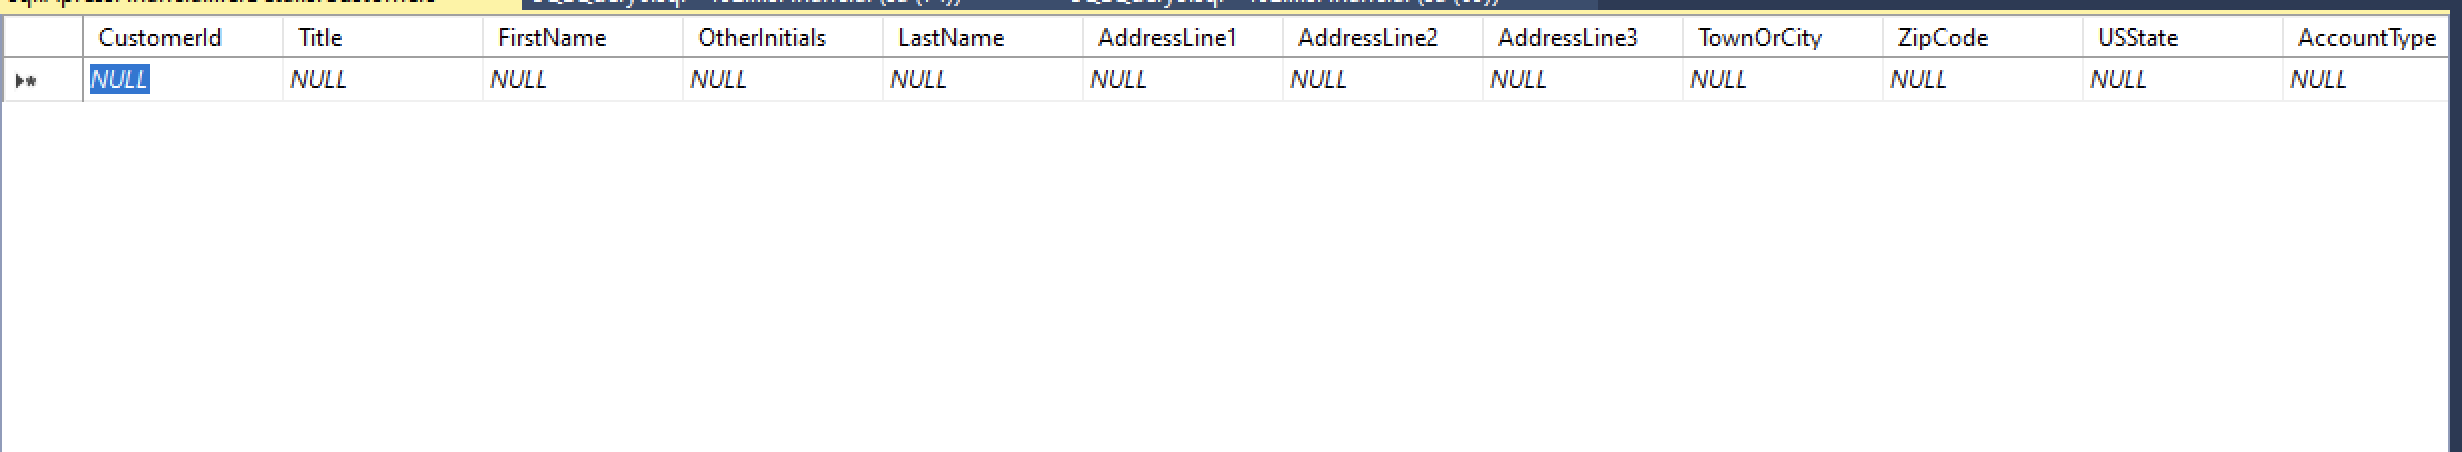
\includegraphics[width=\textwidth]{images/task-1/6.png}
  \caption{Окно редактирования строк}
  \label{fig:task-1-6}
\end{figure}

\begin{figure}[H]
  \centering
  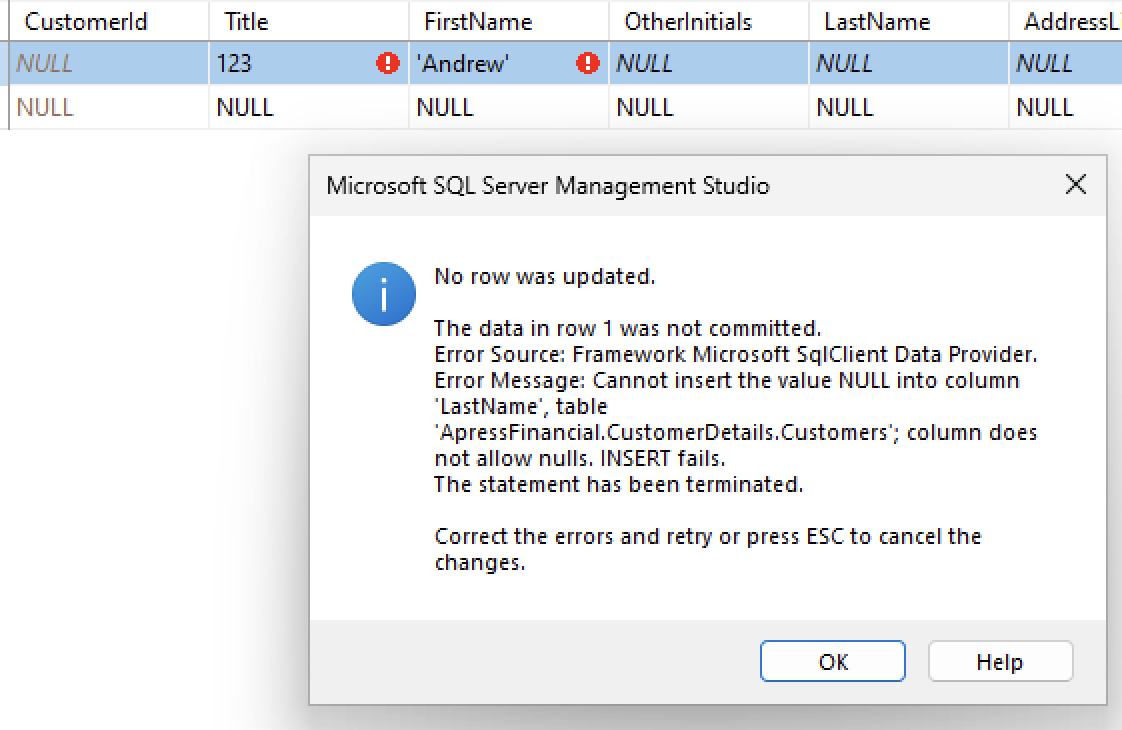
\includegraphics[width=\textwidth]{images/task-1/7.png}
  \caption{Ошибка при добавлении строки с незаполненными обязательными
    столбцами}
  \label{fig:task-1-7}
\end{figure}

\begin{figure}[H]
  \centering
  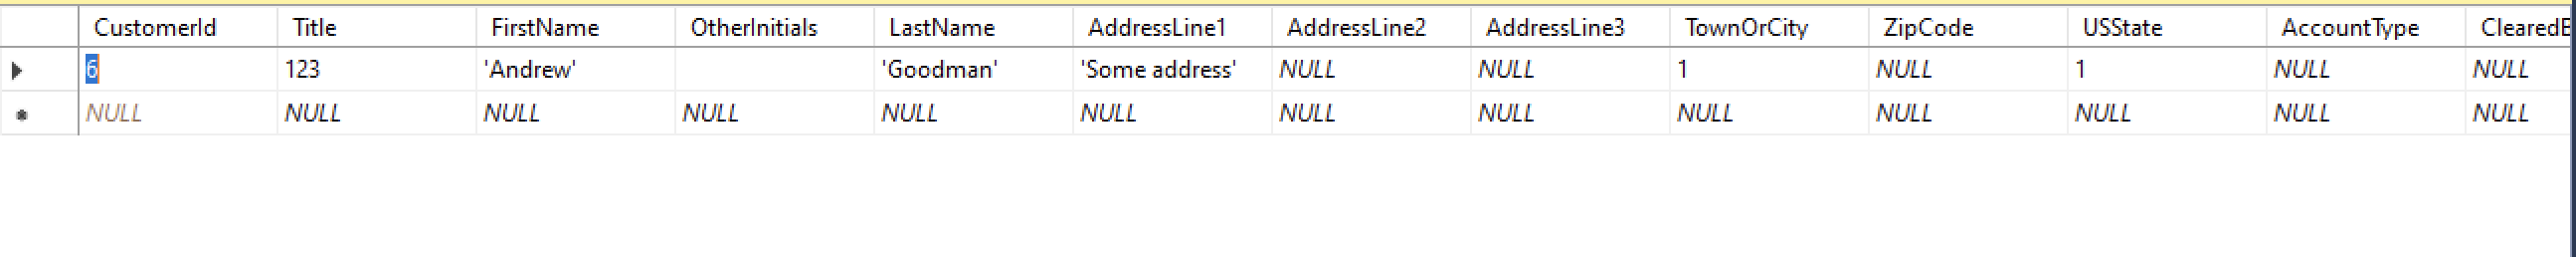
\includegraphics[width=\textwidth]{images/task-1/8.png}
  \caption{Результат добавления строки}
  \label{fig:task-1-8}
\end{figure}

\begin{figure}[H]
  \centering
  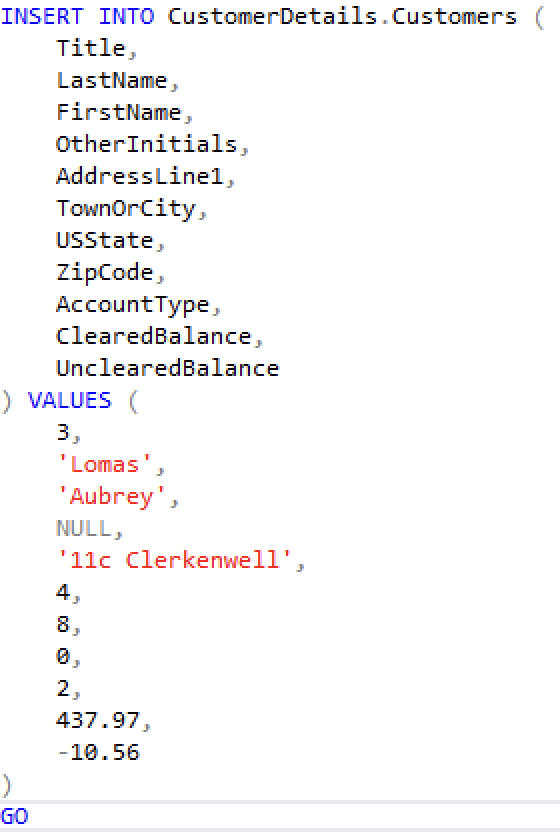
\includegraphics[width=0.6\textwidth]{images/task-1/9.png}
  \caption{Запрос для добавления строки в таблицу}
  \label{fig:task-1-9}
\end{figure}

\subsubsection{Инструкции проверки целостности DDBC}

В запросе, показанном на рисунке \ref{fig:task-1-10}, удаляются все строки
таблицы, а затем с помощью <<\foreignlanguage{english}{DBCC CHECKIDENT}>>
идентификатору <<\foreignlanguage{english}{CustomerId}>> устанавливается
значение 0. Как видно на рисунке \ref{fig:task-1-10}, запрос был успешно
выполнен, обнуление идентификатора прошло успешно.

\begin{figure}[H]
  \centering
  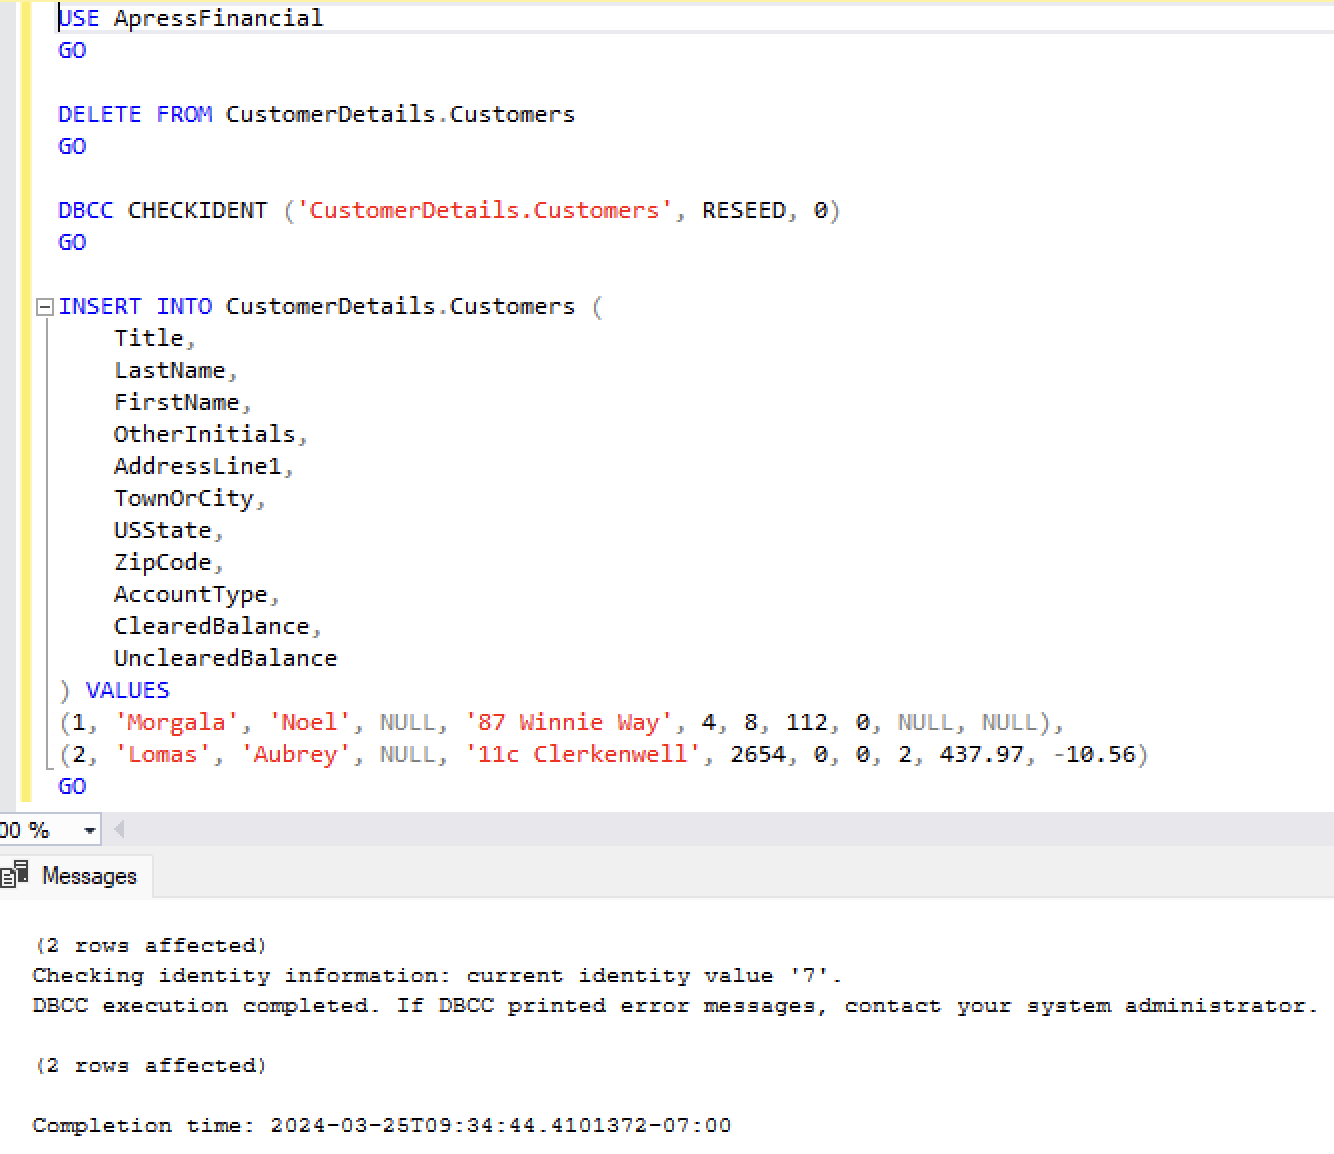
\includegraphics[width=\textwidth]{images/task-1/10.png}
  \caption{Запрос и результат его выполнения}
  \label{fig:task-1-10}
\end{figure}

\subsubsection{Вставка значений в столбцы Identity}

С помощью сценария из файла
<<\foreignlanguage{english}{SQLQuery\_Insert\_to\_Identity.sql}>> (рисунок
\ref{fig:task-1-11}) во временную таблицу были вставлены несколько строк для
проверки работы <<\foreignlanguage{english}{IDENTITY\_INSERT}>>. С помощью
данной директивы можно разрешить вставку идентификаторов в таблицу (вместо
автоматического добавления). Как видно на рисунке \ref{fig:task-1-12},
в таблицу были вставлены ровно те идентификаторы, которые были указаны.

\begin{figure}[H]
  \centering
  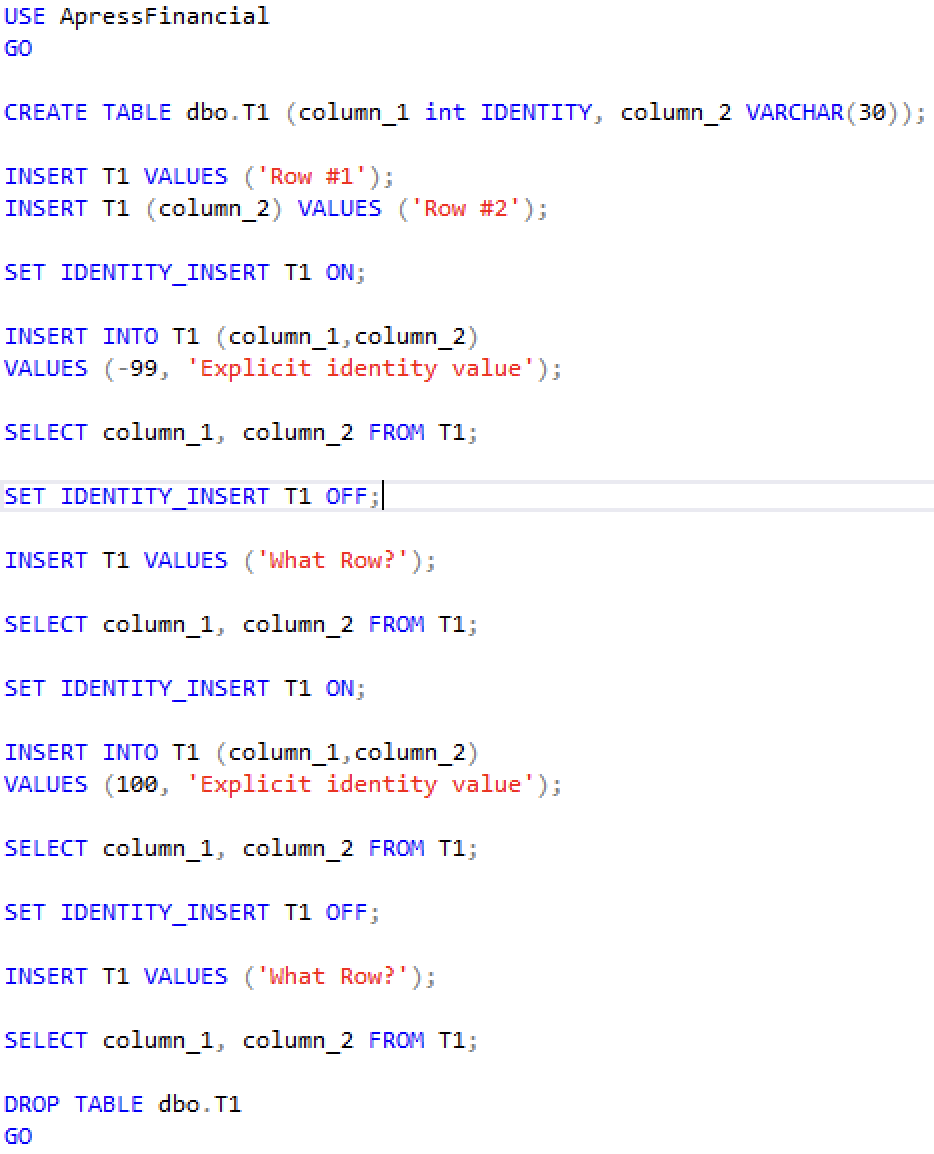
\includegraphics[width=0.8\textwidth]{images/task-1/11.png}
  \caption{
    Запрос для проверки работы <<\foreignlanguage{english}{IDENTITY\_INSERT}>>
  }
  \label{fig:task-1-11}
\end{figure}

\begin{figure}[H]
  \centering
  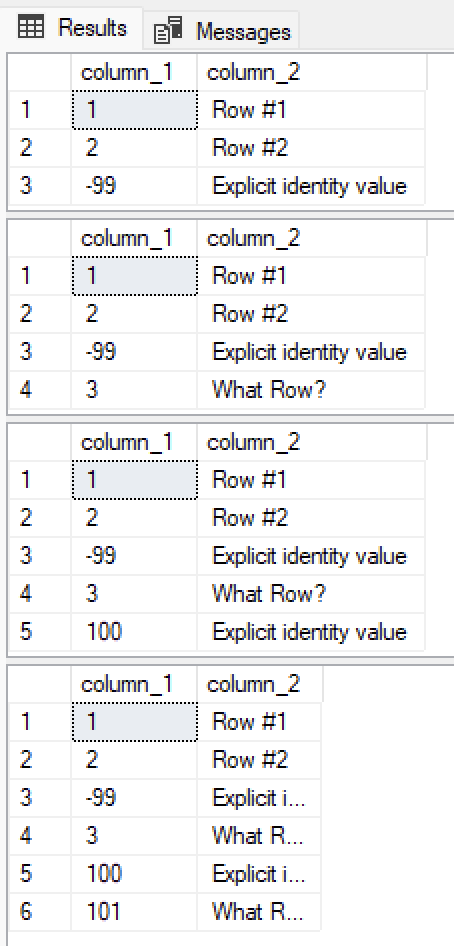
\includegraphics[width=0.4\textwidth]{images/task-1/12.png}
  \caption{Результат выполнения запроса}
  \label{fig:task-1-12}
\end{figure}

\subsubsection{Ограничения для столбцов}

С помощью запроса, показанного на рисунке \ref{fig:task-1-13}, для столбцов
таблицы <<\foreignlanguage{english}{CustomerProducts}>> были установлены
ограничения:
\begin{itemize}
  \item кластеризованный первичный ключ;
  \item ограничение, что <<\foreignlanguage{english}{AmountToCollect}>> больше
  нуля;
  \item значение по умолчанию 0 для <<\foreignlanguage{english}{Renewable}>>.
\end{itemize}
После выполнения данного запроса данные ограничения появились в обозревателе
(рисунок \ref{fig:task-1-14}).

Затем, с помощью кнопки <<\foreignlanguage{english}{Manage Check Constraints}>>
(рисунок \ref{fig:task-1-15}) было открыто окно изменения ограничений (рисунок
\ref{fig:task-1-16}). С помощью кнопки <<\foreignlanguage{english}{Add}>> было
добавлено новое ограничение, которое гарантирует, что дата в
<<\foreignlanguage{english}{LastCollection}>> больше или равна
<<\foreignlanguage{english}{LastCollected}>> (рисунок \ref{fig:task-1-17}).
После сохранения изменений данное ограничение было проверено запросом,
представленном на рисунке \ref{fig:task-1-18}. Как видно на рисунке
\ref{fig:task-1-19}, некорректные (с точки зрения ограничений) данные не были
вставлены в таблицу.

\begin{figure}[H]
  \centering
  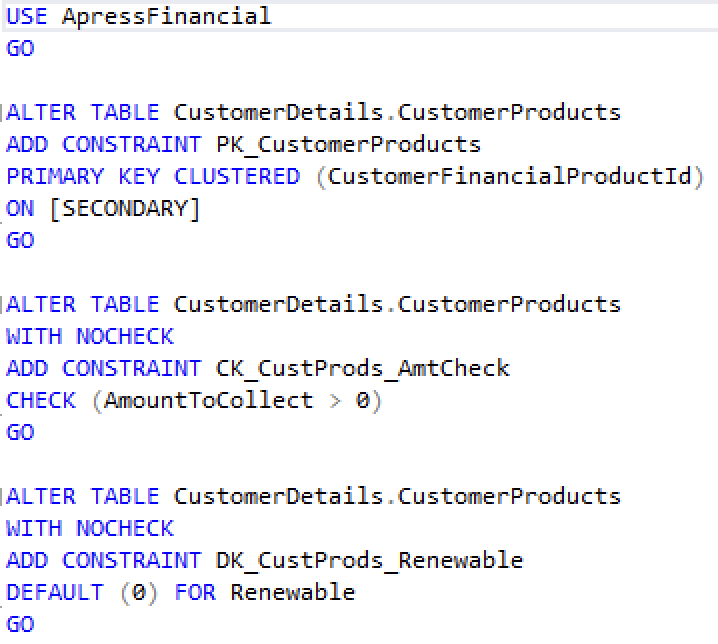
\includegraphics[width=0.6\textwidth]{images/task-1/13.png}
  \caption{Запрос для создания ограничений столбцов таблицы}
  \label{fig:task-1-13}
\end{figure}

\begin{figure}[H]
  \centering
  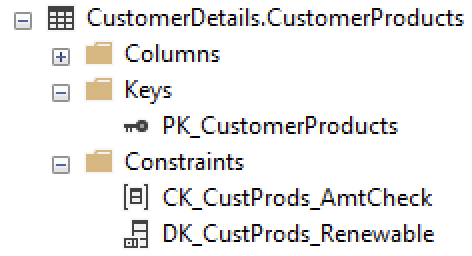
\includegraphics[width=0.4\textwidth]{images/task-1/14.png}
  \caption{Созданные ограничения}
  \label{fig:task-1-14}
\end{figure}

\begin{figure}[H]
  \centering
  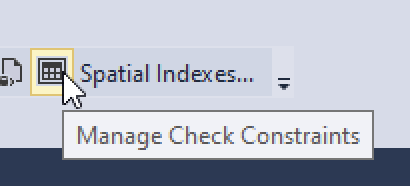
\includegraphics[width=0.4\textwidth]{images/task-1/15.png}
  \caption{Кнопка открытия окна изменения ограничений}
  \label{fig:task-1-15}
\end{figure}

\begin{figure}[H]
  \centering
  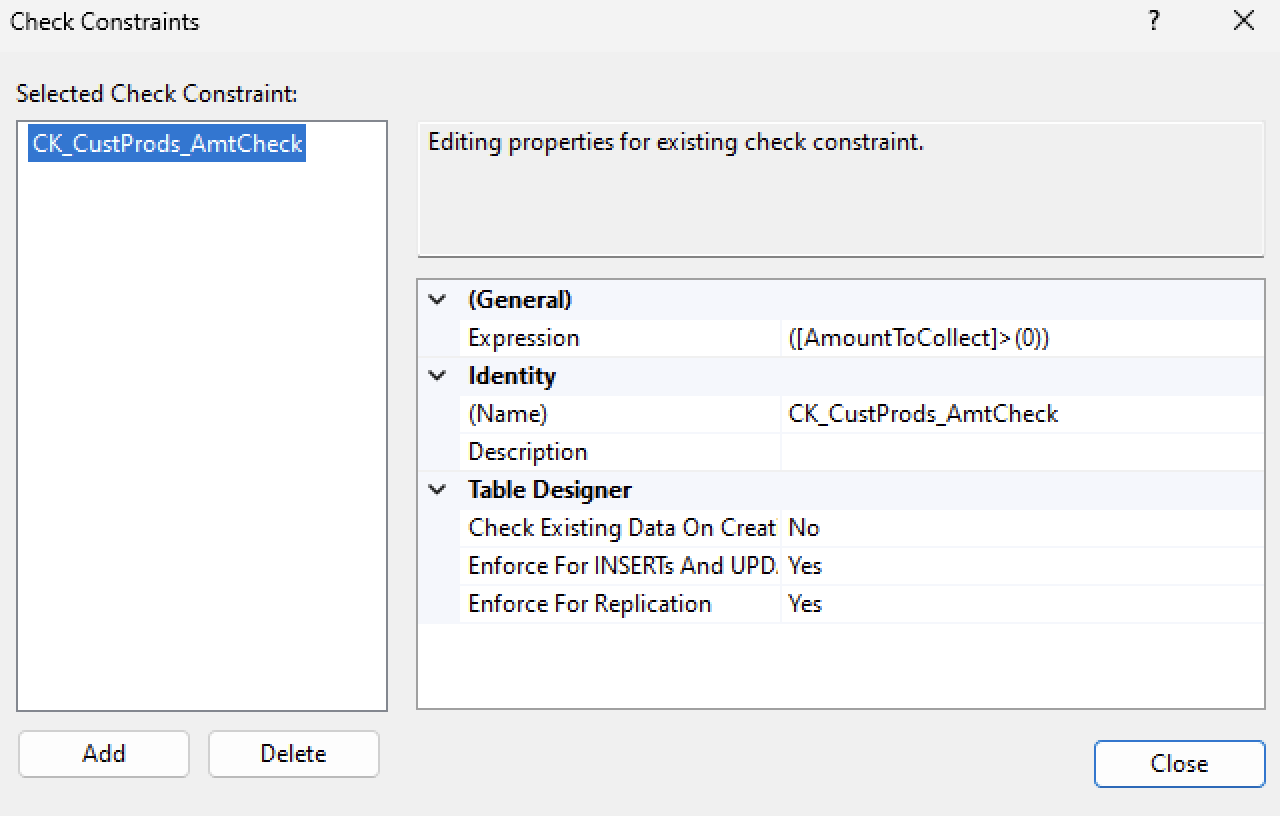
\includegraphics[width=0.8\textwidth]{images/task-1/16.png}
  \caption{Окно изменения ограничений таблицы}
  \label{fig:task-1-16}
\end{figure}

\begin{figure}[H]
  \centering
  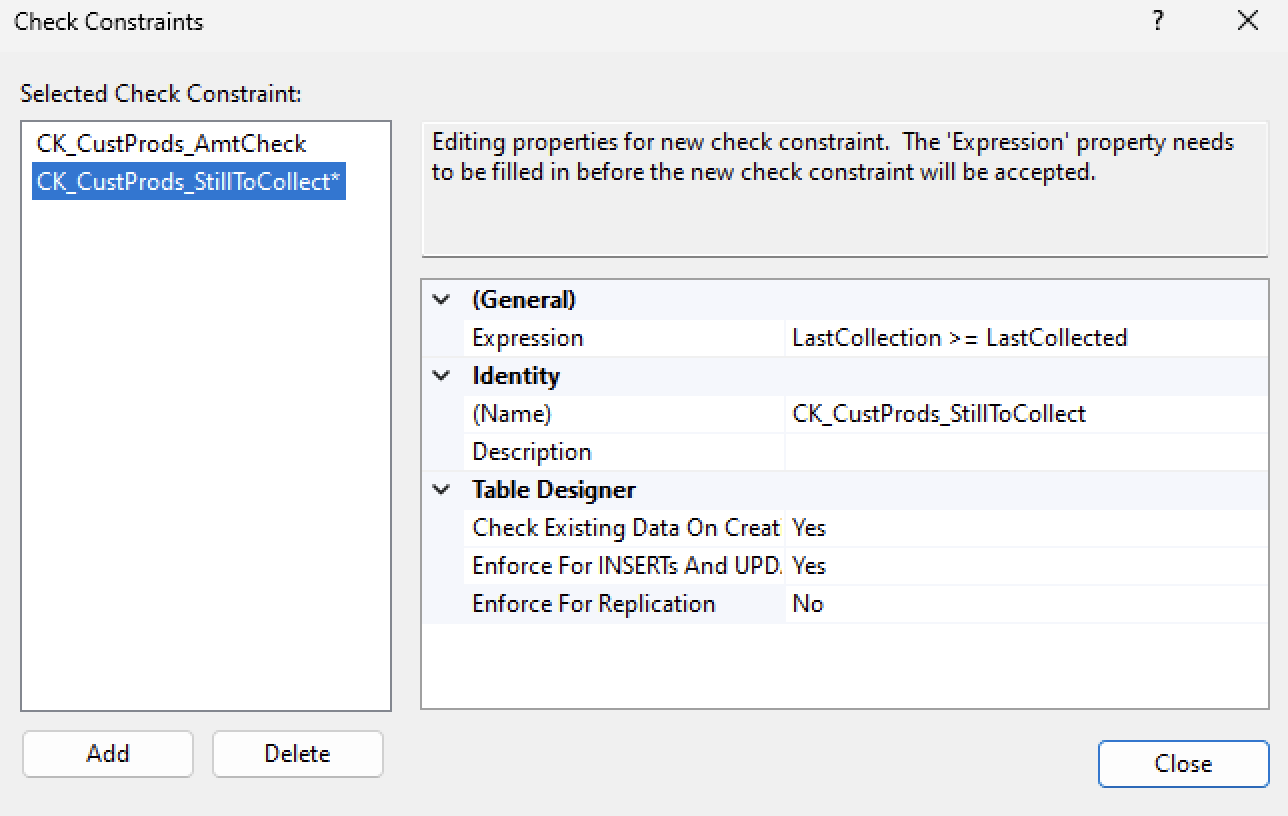
\includegraphics[width=0.8\textwidth]{images/task-1/17.png}
  \caption{Новое ограничение}
  \label{fig:task-1-17}
\end{figure}

\begin{figure}[H]
  \centering
  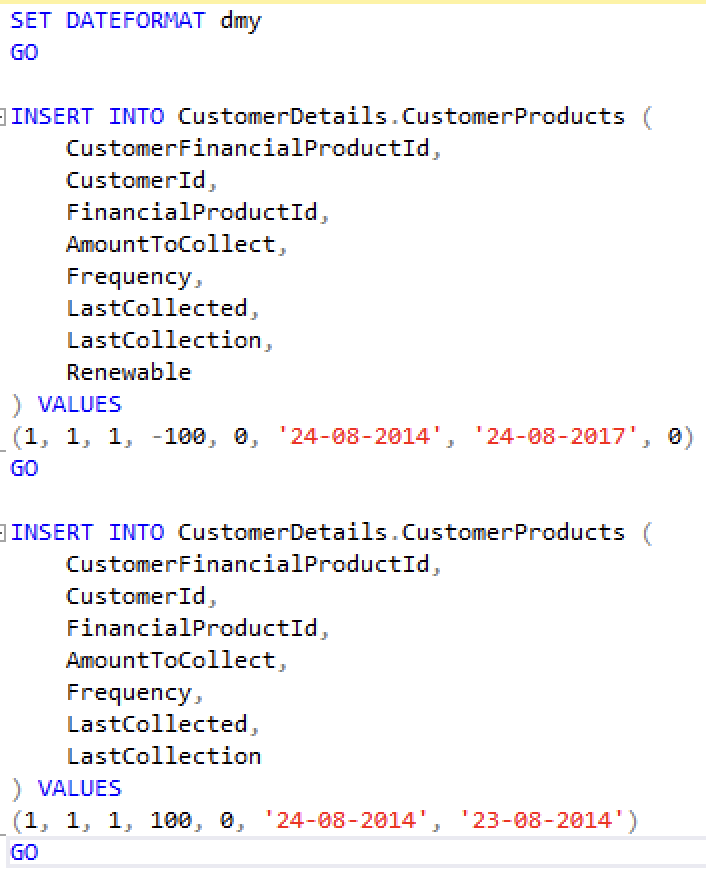
\includegraphics[width=0.7\textwidth]{images/task-1/18.png}
  \caption{Запрос для проверки ограничений}
  \label{fig:task-1-18}
\end{figure}

\begin{figure}[H]
  \centering
  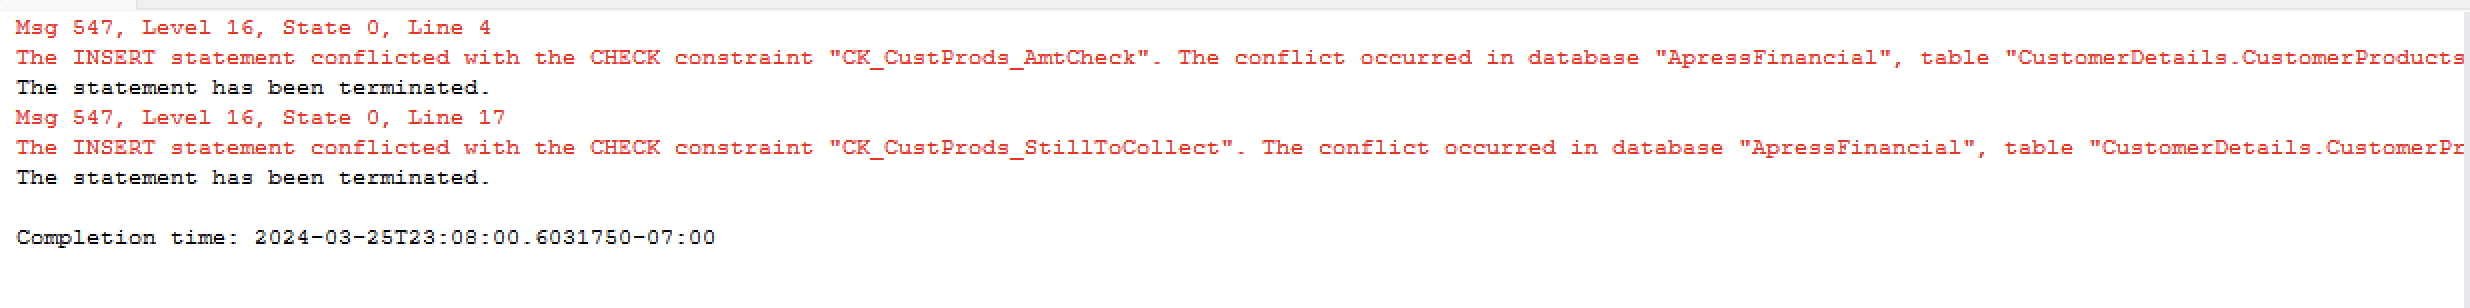
\includegraphics[width=\textwidth]{images/task-1/19.png}
  \caption{Результат выполнения запроса}
  \label{fig:task-1-19}
\end{figure}

\subsubsection{Одновременная вставка нескольких записей}

С помощью запроса, показанного на рисунке \ref{fig:task-1-20}, в таблицу
<<\foreignlanguage{english}{Customers}>> было вставлено несколько записей с
помощью одного <<\foreignlanguage{english}{INSERT INTO}>>. Как видно на рисунке
\ref{fig:task-1-21}, данные были успешно вставлены в таблицу.

\begin{figure}[H]
  \centering
  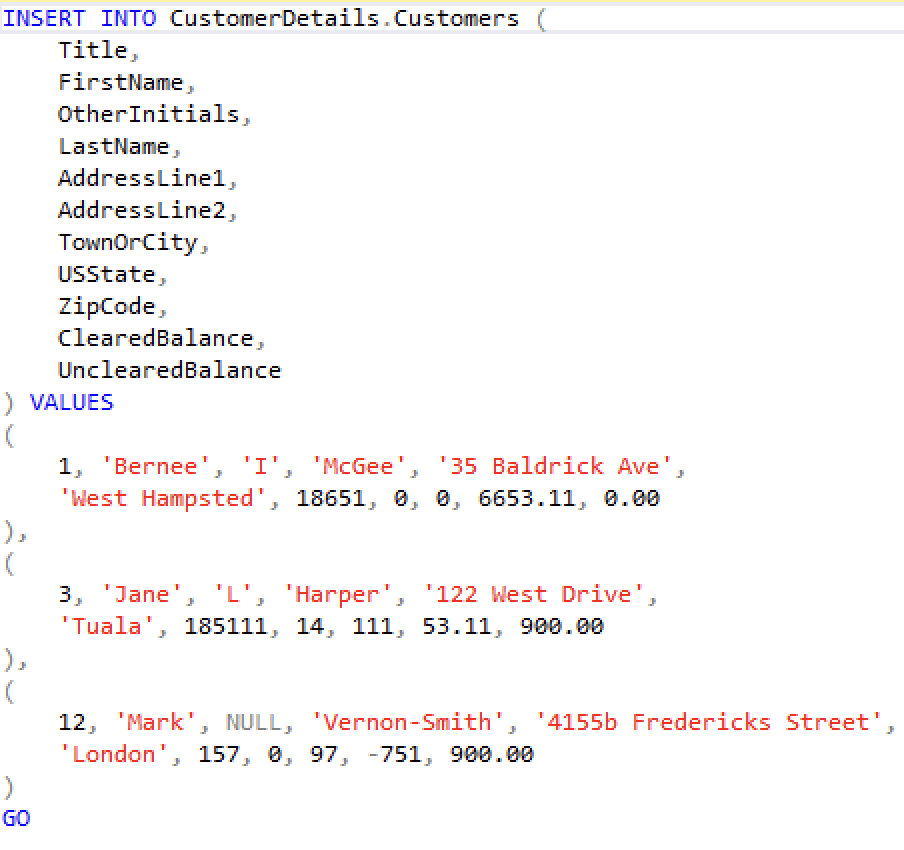
\includegraphics[width=0.8\textwidth]{images/task-1/20.png}
  \caption{Вставка нескольких записей}
  \label{fig:task-1-20}
\end{figure}

\begin{figure}[H]
  \centering
  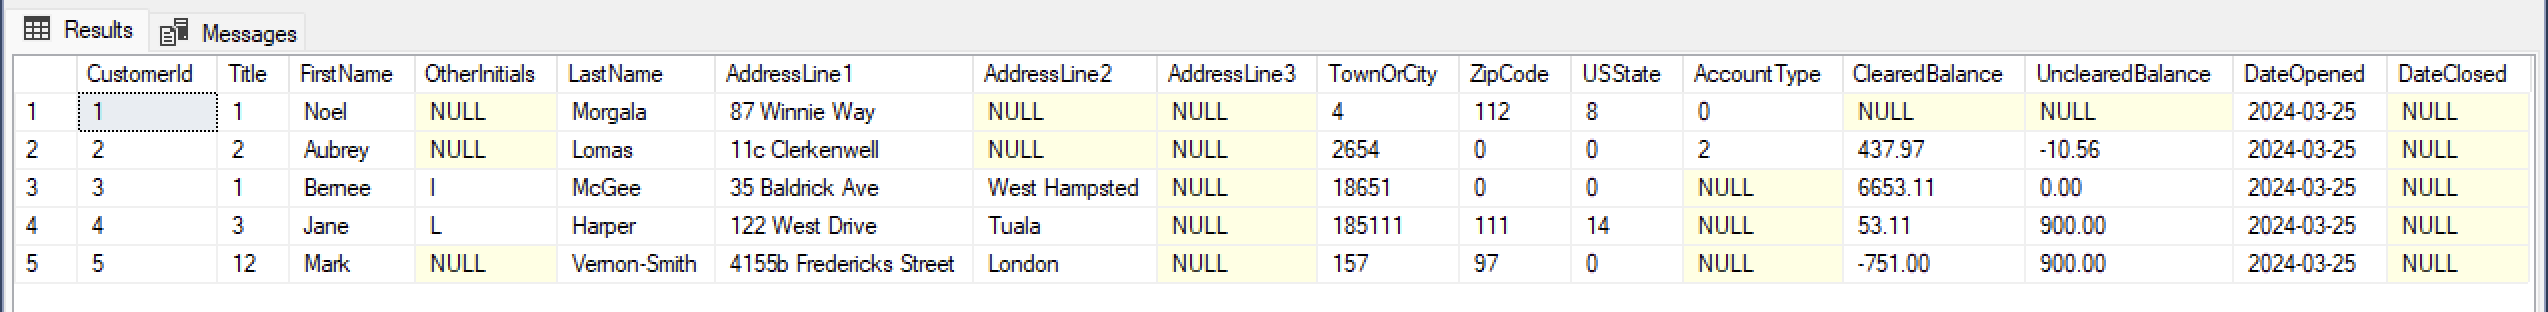
\includegraphics[width=\textwidth]{images/task-1/21.png}
  \caption{Результат добавления данных}
  \label{fig:task-1-21}
\end{figure}

\subsubsection{Заполнение таблиц учебной БД тестовыми данными}

С помощью сценария <<\foreignlanguage{english}{SQLQuery\_BulkInsert.sql}>> в
базу данных были вставлены тестовые данные для дальнейшего тестирования. При
выполнении запроса ошибок не произошло, все данные были успешно добавлены.

\subsubsection{Извлечение данных}

С помощью запроса, показанного на рисунке \ref{fig:task-1-22}, были извлечены
данные из таблицы <<\foreignlanguage{english}{Customers}>> (рисунок
\ref{fig:task-1-23}). После этого с помощью кнопки
<<\foreignlanguage{english}{Results To Text}>> в меню
<<\foreignlanguage{english}{Query}>> представление было изменено на текстовое,
как это показано на рисунке \ref{fig:task-1-24}.

\begin{figure}[H]
  \centering
  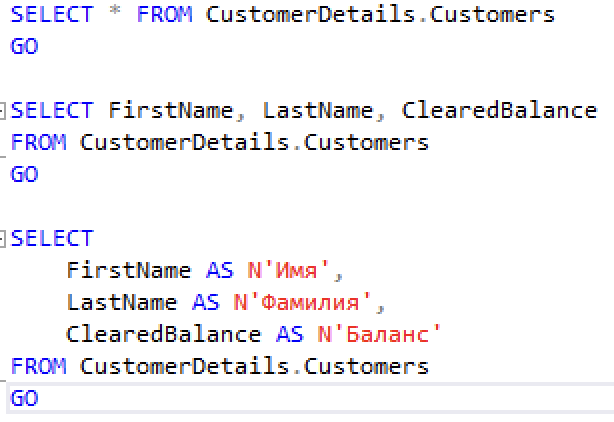
\includegraphics[width=0.7\textwidth]{images/task-1/22.png}
  \caption{Запрос для извлечения данных}
  \label{fig:task-1-22}
\end{figure}

\begin{figure}[H]
  \centering
  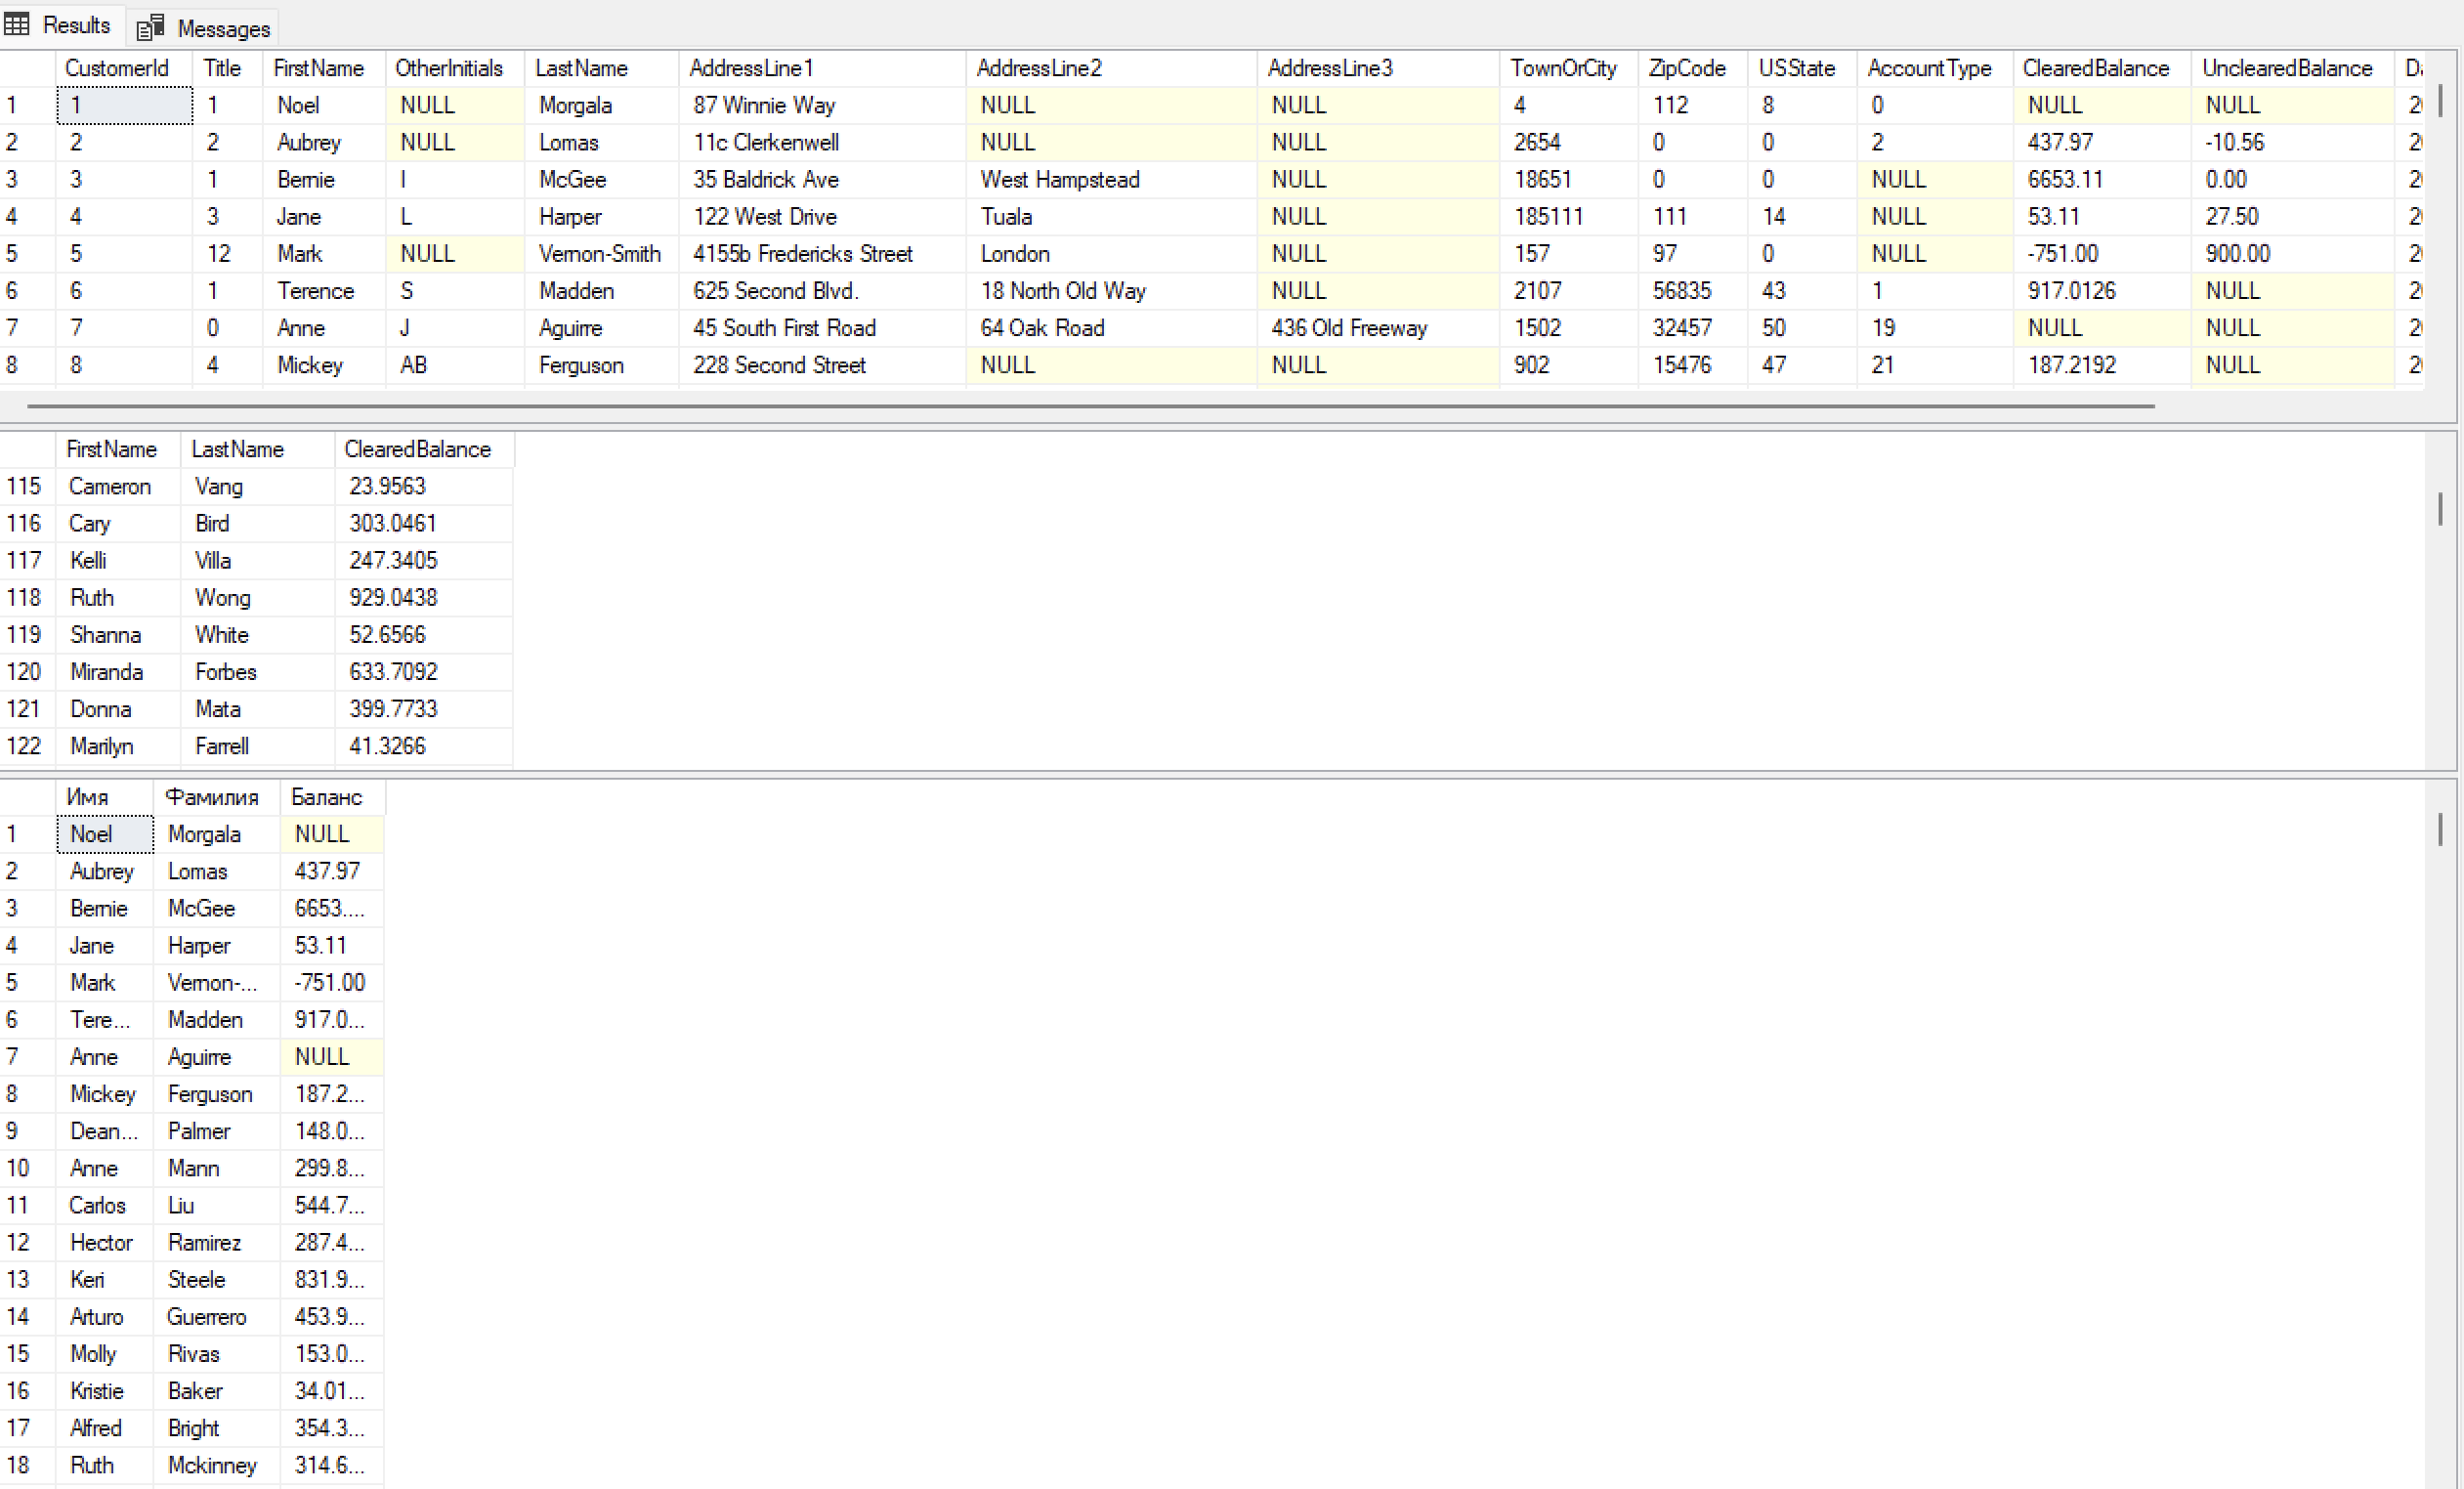
\includegraphics[width=\textwidth]{images/task-1/23.png}
  \caption{Результат выполнения запроса}
  \label{fig:task-1-23}
\end{figure}

\begin{figure}[H]
  \centering
  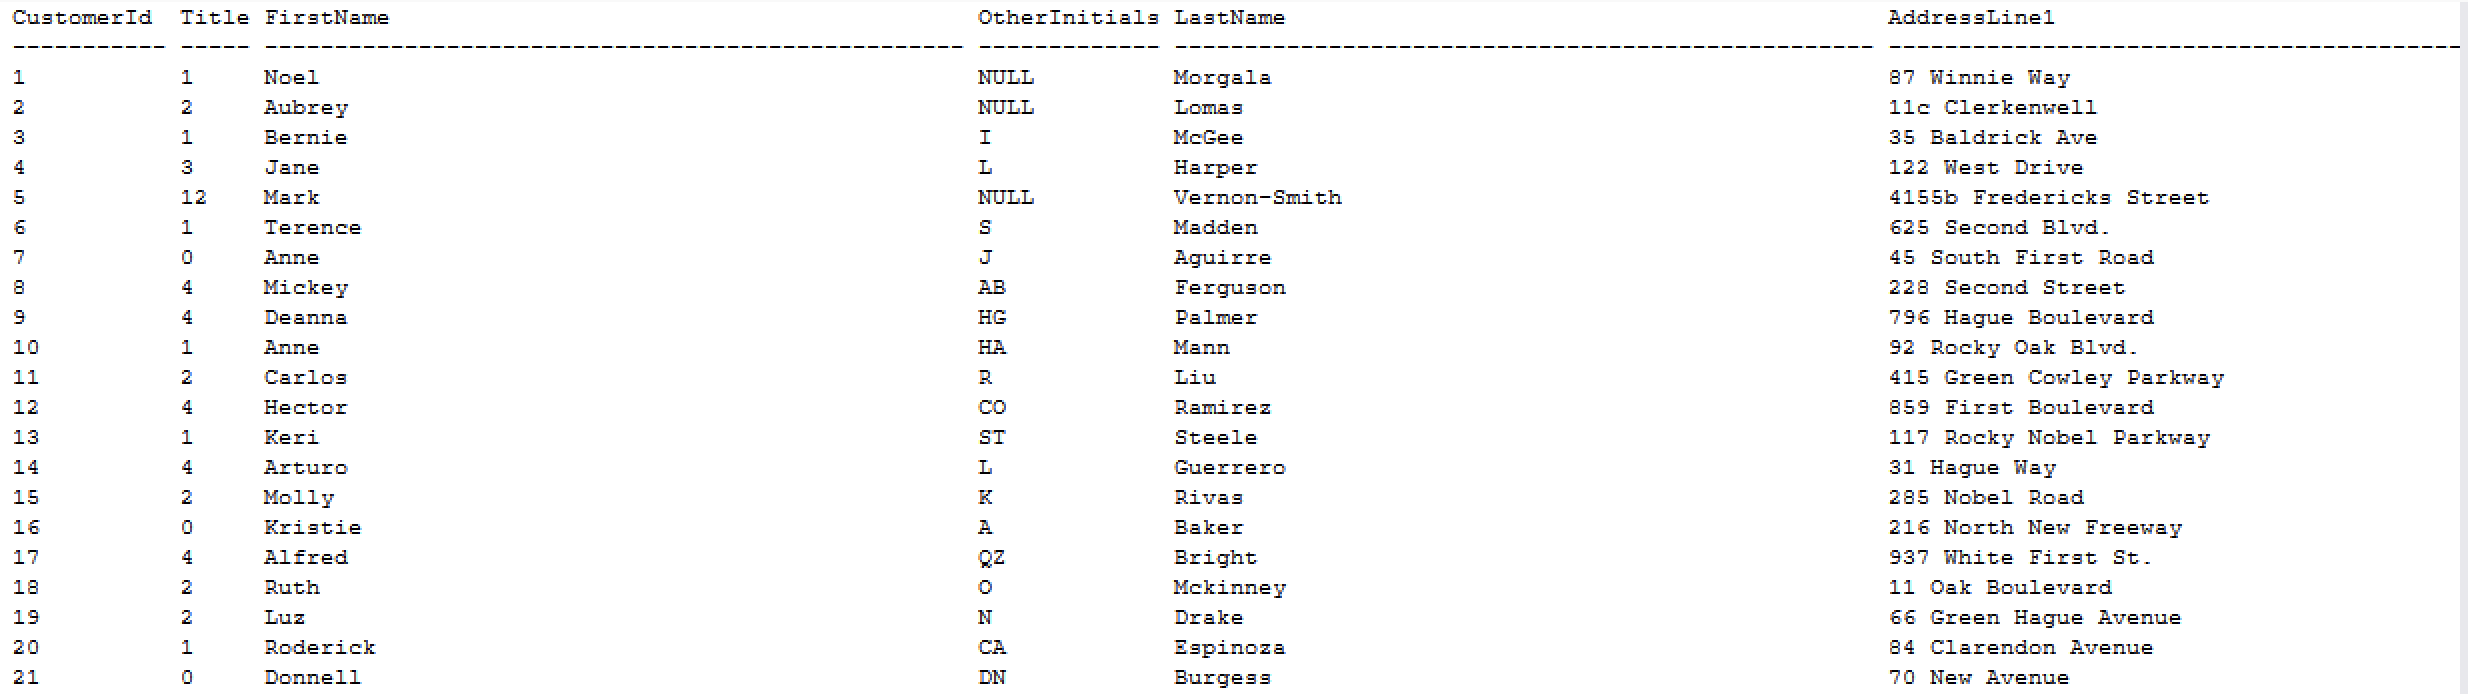
\includegraphics[width=\textwidth]{images/task-1/24.png}
  \caption{Результат выполнения запроса в текстовом виде}
  \label{fig:task-1-24}
\end{figure}

\subsection{Вторая задача}

\subsubsection{Простое обновление данных}

С помощью запроса, показанного на рисунке \ref{fig:task-2-1}, была изменена
фамилия у строки с <<\foreignlanguage{english}{CustomerId}>> равной 7. Как
видно на рисунке \ref{fig:task-2-2}, фамилия была успешно изменена.

\begin{figure}[H]
  \centering
  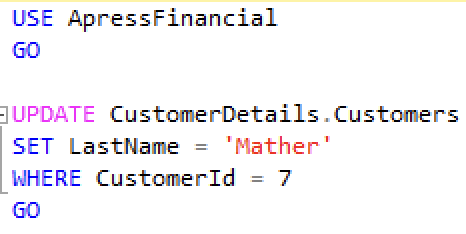
\includegraphics[width=0.5\textwidth]{images/task-2/1.png}
  \caption{Запрос на обновление данных}
  \label{fig:task-2-1}
\end{figure}

\begin{figure}[H]
  \centering
  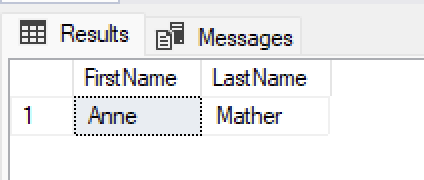
\includegraphics[width=0.5\textwidth]{images/task-2/2.png}
  \caption{Результат обновления данных}
  \label{fig:task-2-2}
\end{figure}

\subsubsection{Обновление данных с помощью переменной}

В запросе, который показан на рисунке \ref{fig:task-2-3}, используется
переменная, а также другие столбцы таблицы для изменения данных в таблице. Так,
с помощью переменной <<\foreignlanguage{english}{ValueToUpdate}>> изменяется
фамилия клиента, а с помощью переменной
<<\foreignlanguage{english}{UnclearedBalance}>> обновляется баланс клиента. Как
видно на рисунке \ref{fig:task-2-4}, данные были успешно обновлены в
соответствии с ожидаемым результатом.

\begin{figure}[H]
  \centering
  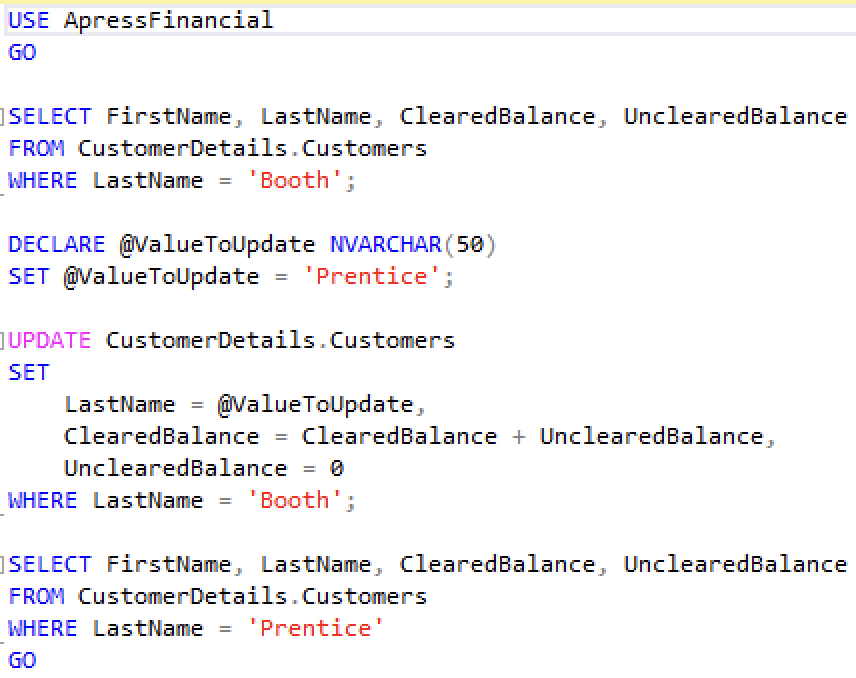
\includegraphics[width=0.9\textwidth]{images/task-2/3.png}
  \caption{Запрос на обновление данных}
  \label{fig:task-2-3}
\end{figure}

\begin{figure}[H]
  \centering
  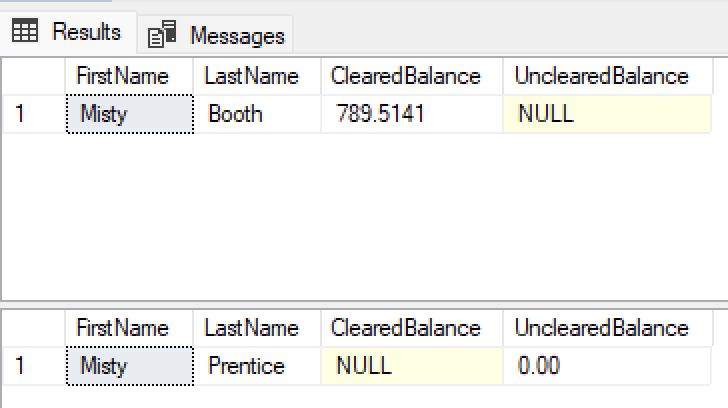
\includegraphics[width=0.7\textwidth]{images/task-2/4.png}
  \caption{Результат обновления данных}
  \label{fig:task-2-4}
\end{figure}

\subsubsection{Преобразование данных при обновлении}

На рисунке \ref{fig:task-2-5} показан пример запроса, при выполнении которого
происходит неявное преобразование типа данных. При выполнении данного запроса,
что видно из рисунка \ref{fig:task-2-6}, строковый тип был преобразован в
денежный тип, поскольку, на самом деле, в строке лежало число. Однако, если в
строке будет лежать что-то отличное от числа, например, как это показано на
рисунке \ref{fig:task-2-7}, то возникнет ошибка (рисунок \ref{fig:task-2-8}).

\begin{figure}[H]
  \centering
  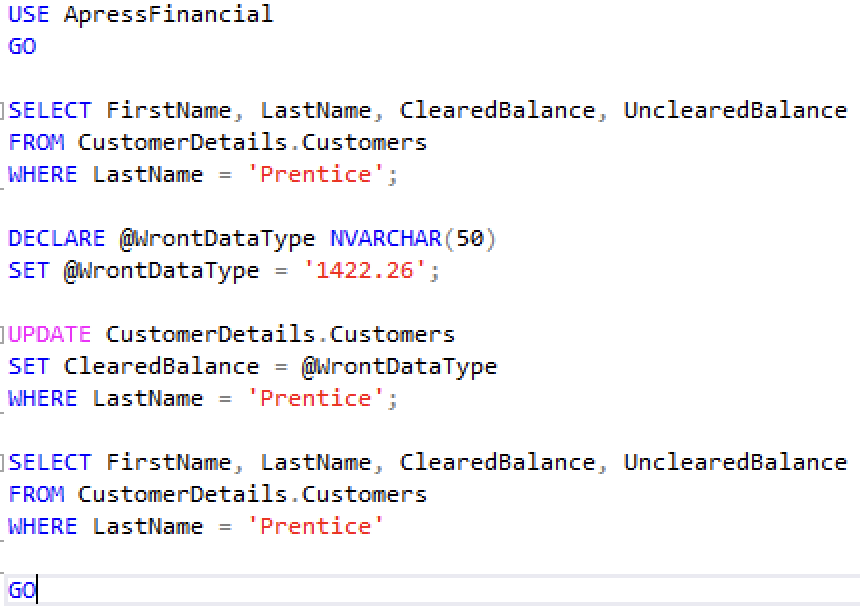
\includegraphics[width=0.8\textwidth]{images/task-2/5.png}
  \caption{Запрос на обновление данных}
  \label{fig:task-2-5}
\end{figure}

\begin{figure}[H]
  \centering
  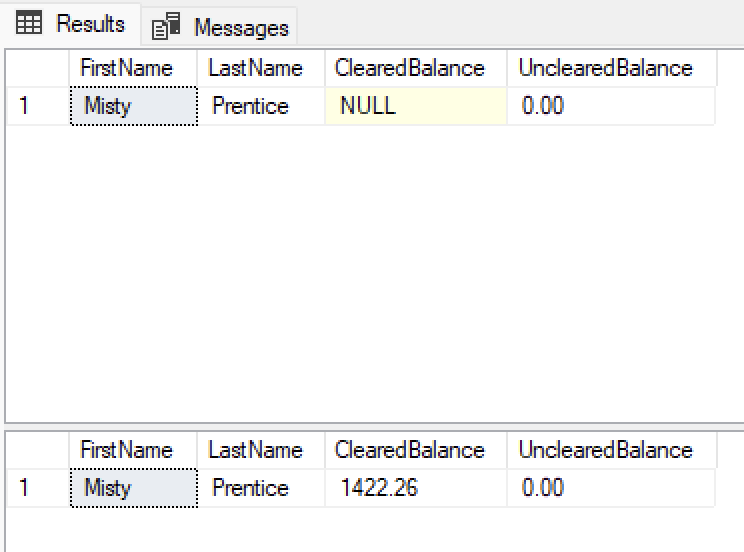
\includegraphics[width=0.7\textwidth]{images/task-2/6.png}
  \caption{Результат обновления данных}
  \label{fig:task-2-6}
\end{figure}

\begin{figure}[H]
  \centering
  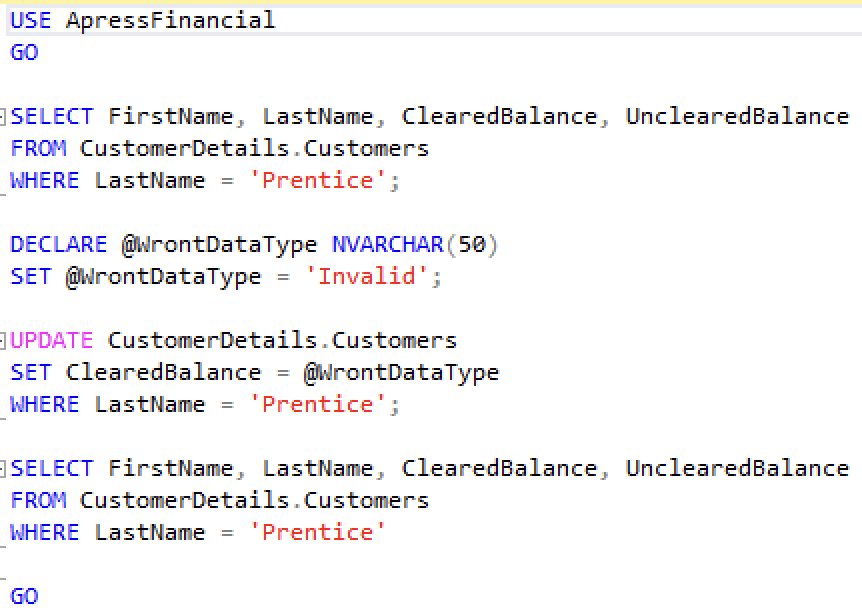
\includegraphics[width=0.8\textwidth]{images/task-2/7.png}
  \caption{Некорректный запрос на обновление данных}
  \label{fig:task-2-7}
\end{figure}

\begin{figure}[H]
  \centering
  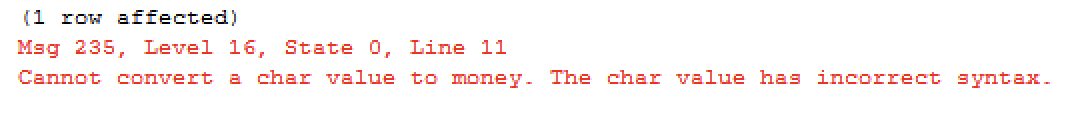
\includegraphics[width=\textwidth]{images/task-2/8.png}
  \caption{Результат выполнения некорректного запроса}
  \label{fig:task-2-8}
\end{figure}

\subsection{Третья задача}

\subsubsection{Создание временной таблицы}

С помощью запроса, показанного на рисунке \ref{fig:task-3-1}, была создана
временная таблица данных <<\foreignlanguage{english}{CustTemp}>>, содержащая 5
первых строк из таблицы <<\foreignlanguage{english}{Customers}>>. Как видно на
рисунке \ref{fig:task-3-2}, запрос был успешно выполнен.

\begin{figure}[H]
  \centering
  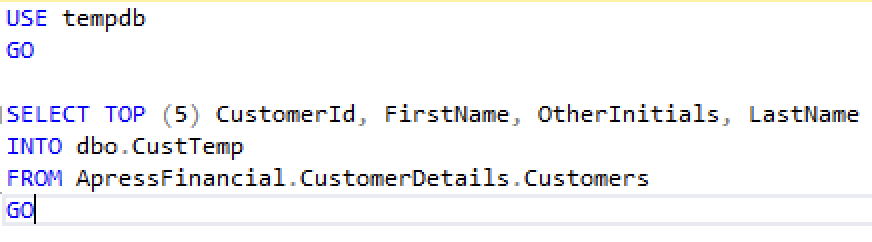
\includegraphics[width=0.8\textwidth]{images/task-3/1.png}
  \caption{Запрос на создание временной таблицы}
  \label{fig:task-3-1}
\end{figure}

\begin{figure}[H]
  \centering
  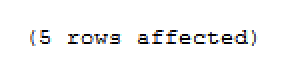
\includegraphics[width=0.3\textwidth]{images/task-3/2.png}
  \caption{Результат выполнения запроса}
  \label{fig:task-3-2}
\end{figure}

\subsubsection{Поведение счетчика идентификаторов при удалении строк}

После выполнения запроса, показанного на рисунке \ref{fig:task-3-3}, из
временной таблицы была удалена строка с
<<\foreignlanguage{english}{CustomerId}>> равным 4. При выполнении запроса,
показанного на рисунке \ref{fig:task-3-4}, как видно на рисунке
\ref{fig:task-3-5}, новая строка получила
<<\foreignlanguage{english}{CustomerId}>> равный 6. Также, при полном удалении
всех строк таблицы с помощью <<\foreignlanguage{english}{DELETE FROM}>> и добавлении новой строки (рисунок \ref{fig:task-3-6}),
счетчик идентификаторов не обнуляется (рисунок \ref{fig:task-3-7}).

\begin{figure}[H]
  \centering
  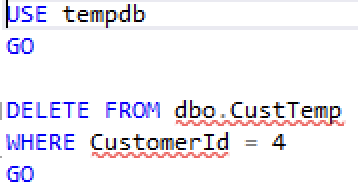
\includegraphics[width=0.4\textwidth]{images/task-3/3.png}
  \caption{Запрос на удаление строки}
  \label{fig:task-3-3}
\end{figure}

\begin{figure}[H]
  \centering
  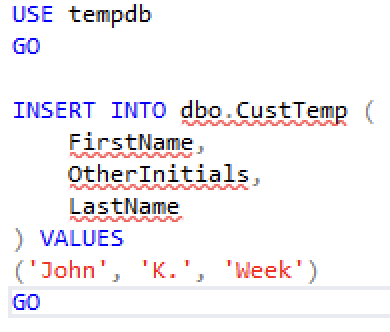
\includegraphics[width=0.4\textwidth]{images/task-3/4.png}
  \caption{Запрос на создание строки}
  \label{fig:task-3-4}
\end{figure}

\begin{figure}[H]
  \centering
  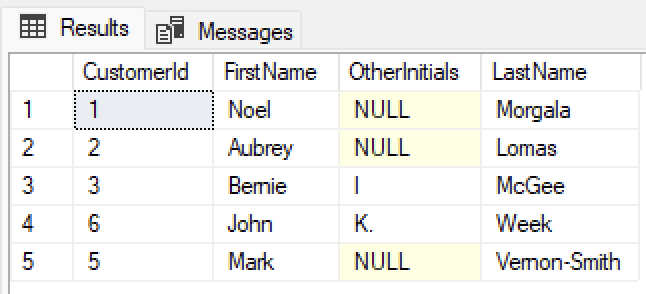
\includegraphics[width=0.7\textwidth]{images/task-3/5.png}
  \caption{Результат выполнения запросов}
  \label{fig:task-3-5}
\end{figure}

\begin{figure}[H]
  \centering
  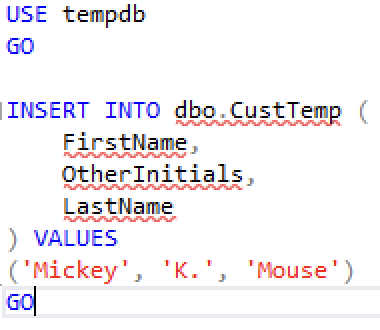
\includegraphics[width=0.4\textwidth]{images/task-3/6.png}
  \caption{Запрос на создание строки после удаления всех строк}
  \label{fig:task-3-6}
\end{figure}

\begin{figure}[H]
  \centering
  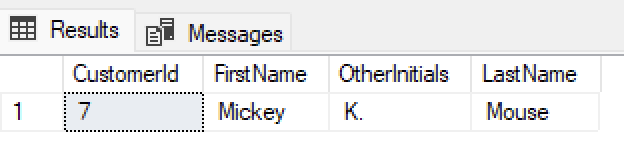
\includegraphics[width=0.8\textwidth]{images/task-3/7.png}
  \caption{Результат выполнения запроса}
  \label{fig:task-3-7}
\end{figure}

\subsubsection{Очистка таблицы}

При использовании <<\foreignlanguage{english}{TRUNCATE TABLE}>>, как это
показано на рисунке \ref{fig:task-3-8}, таблица будет полностью очищена, а также
будет обнулен счетчик идентификатора. Это можно проверить с помощью запроса,
показанного на рисунке \ref{fig:task-3-9}. После выполнения запроса в таблицу
была добавлена новая строка, идентификатор которой равен 1 (рисунок
\ref{fig:task-3-10}).

\begin{figure}[H]
  \centering
  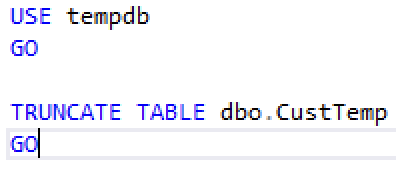
\includegraphics[width=0.4\textwidth]{images/task-3/8.png}
  \caption{Запрос для очистки таблицы}
  \label{fig:task-3-8}
\end{figure}

\begin{figure}[H]
  \centering
  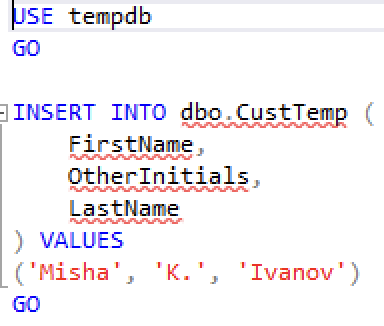
\includegraphics[width=0.4\textwidth]{images/task-3/9.png}
  \caption{Запрос на создание новой строки}
  \label{fig:task-3-9}
\end{figure}

\begin{figure}[H]
  \centering
  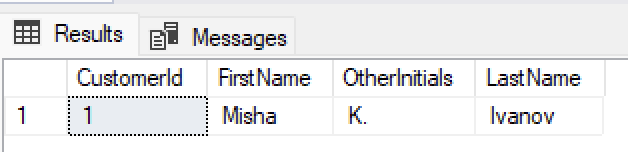
\includegraphics[width=0.8\textwidth]{images/task-3/10.png}
  \caption{Созданная строка}
  \label{fig:task-3-10}
\end{figure}

\subsection{Четвертая задача}

\subsubsection{Создание недостающих связей}

С помощью скрипта, показанного на рисунке \ref{fig:task-4-1}, были созданы
отсутствующие связи между таблицами. В итоге, получилась диаграмма, показанная
на рисунке \ref{fig:task-4-2}.

\begin{figure}[H]
  \centering
  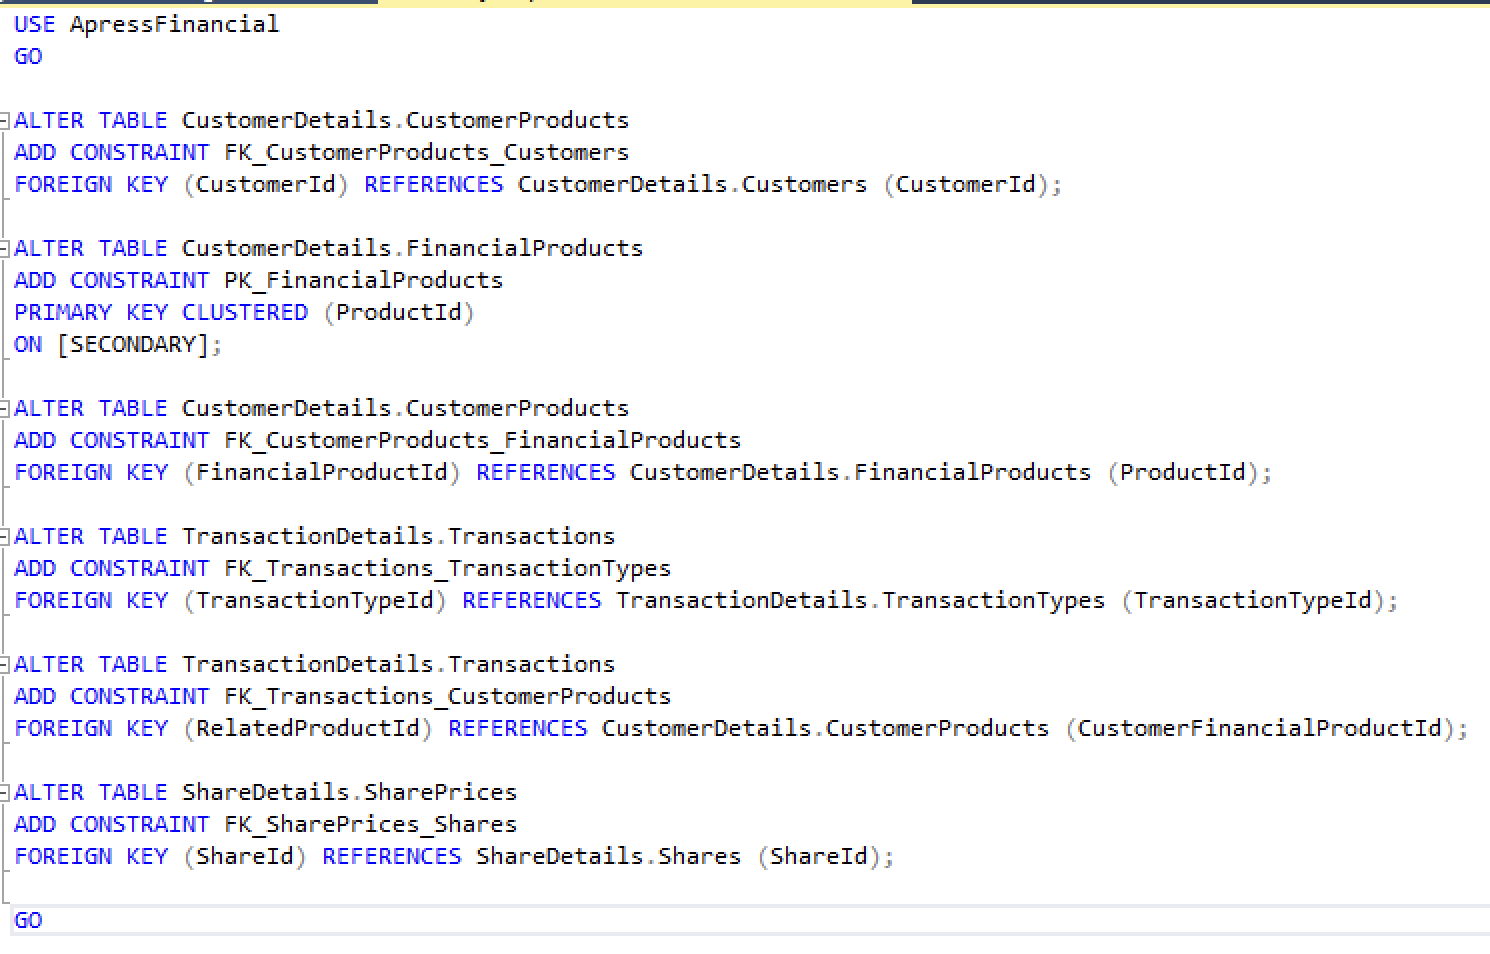
\includegraphics[width=\textwidth]{images/task-4/1.png}
  \caption{Запрос на создания связей}
  \label{fig:task-4-1}
\end{figure}

\begin{figure}[H]
  \centering
  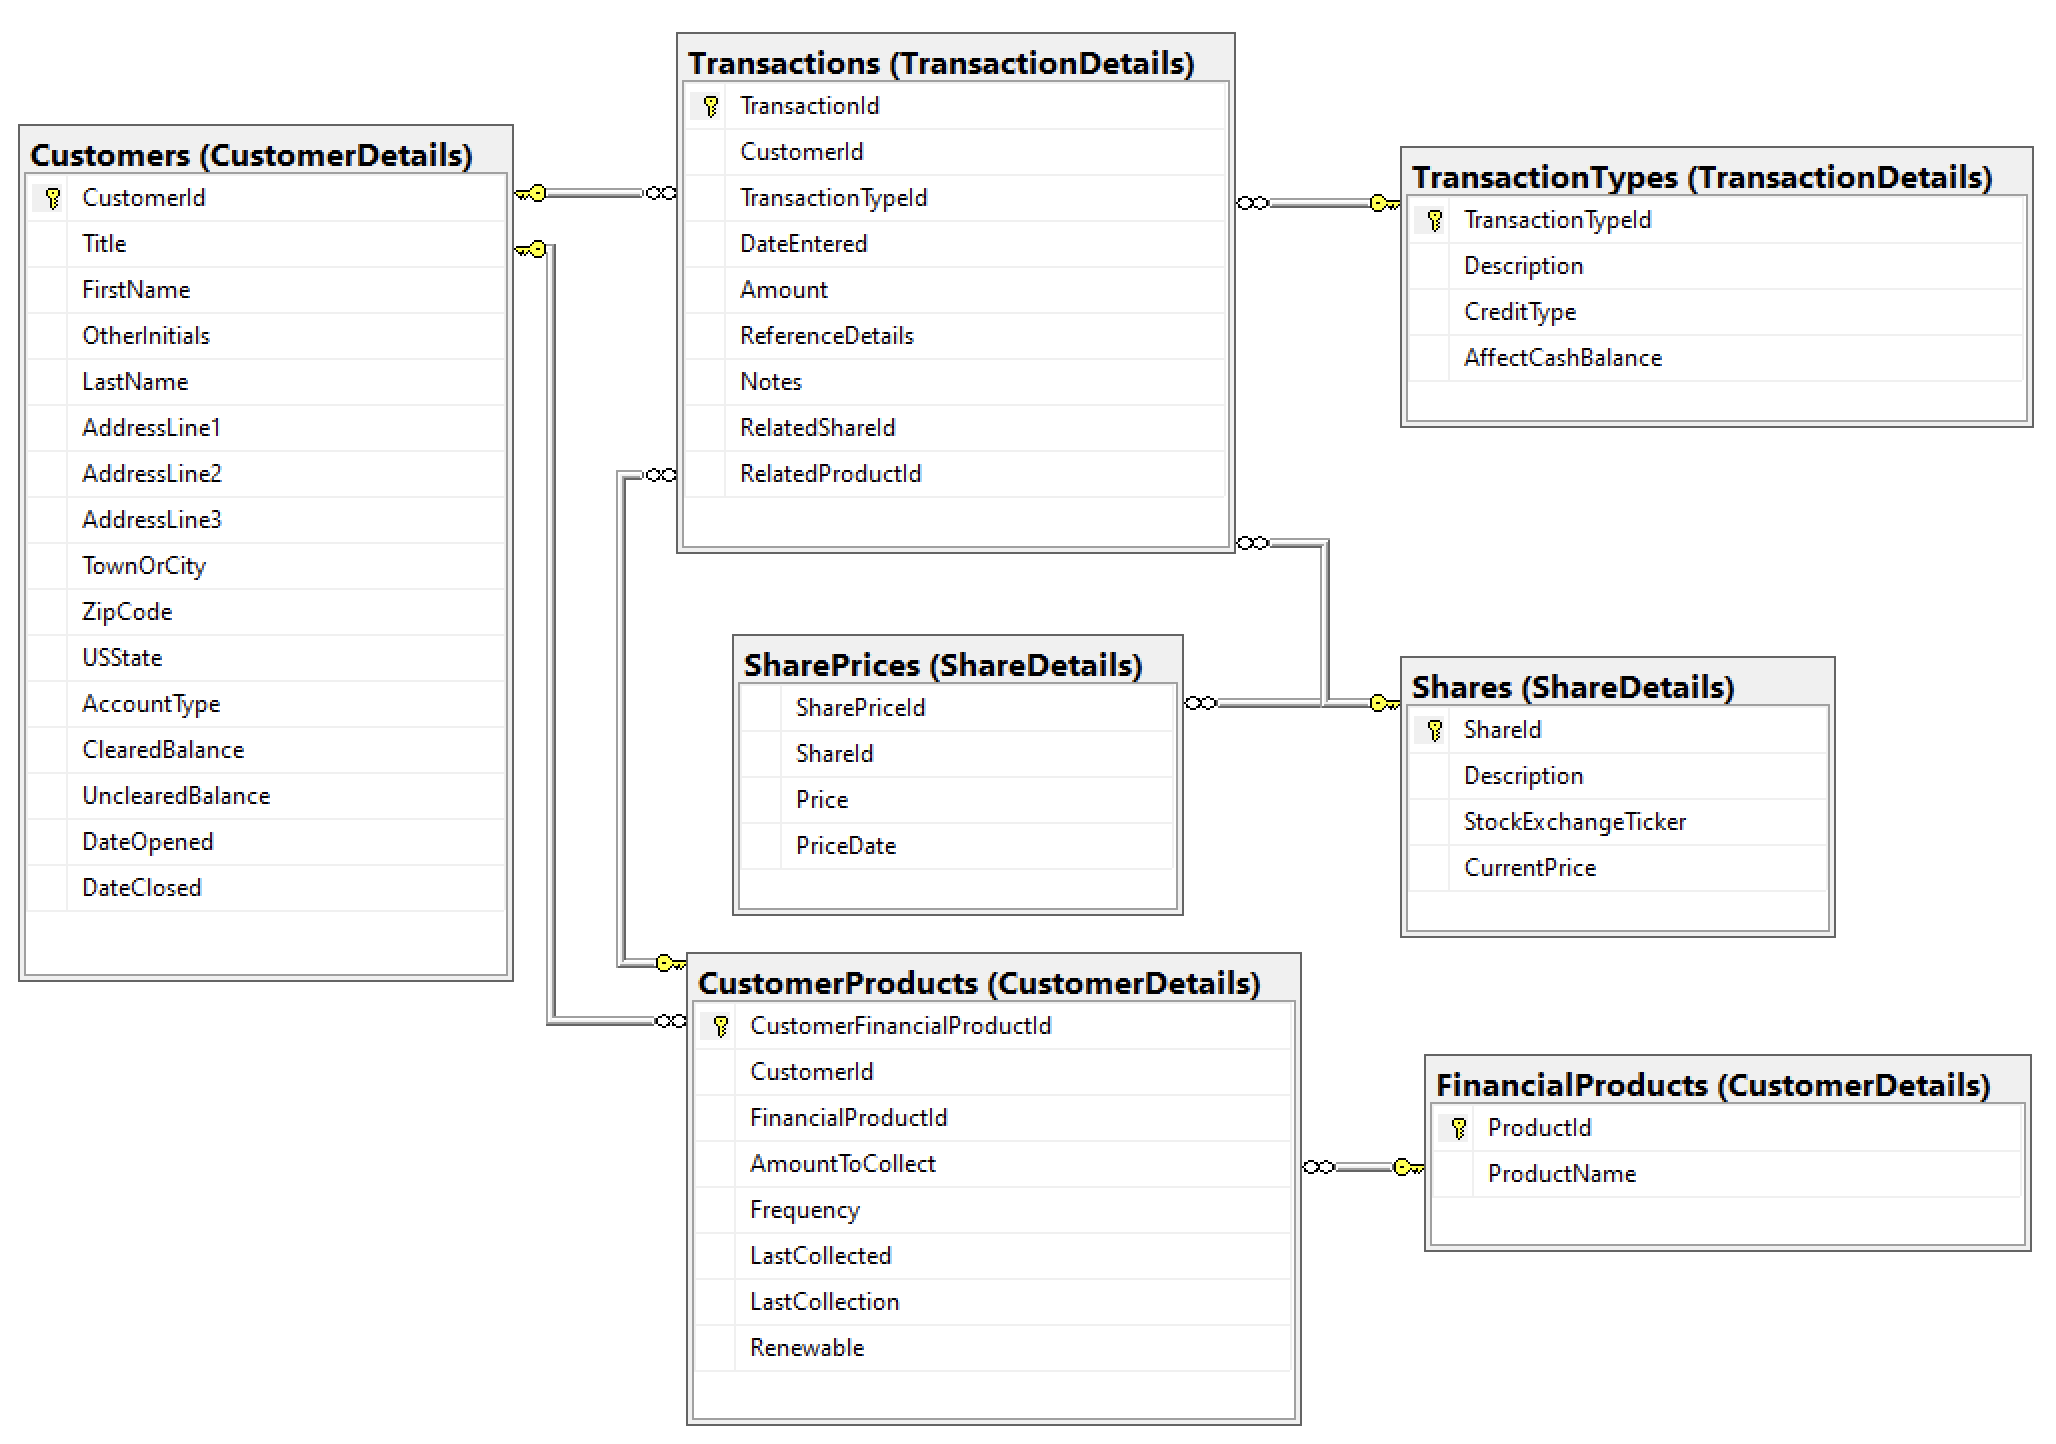
\includegraphics[width=\textwidth]{images/task-4/2.png}
  \caption{Схема связей таблиц в базе данных}
  \label{fig:task-4-2}
\end{figure}

\section{Выводы и анализ результатов работы}

В данной лабораторной работе изучены способы обработки данных в SSMS. Цель,
поставленная в начале работы, достигнута, задачи выполнены.

\end{document}
